% \subsection{Differentially Private Distributed Deep Learning}
% Experiments have been made on benchmark datasets to 1) study the effect of privacy level on the classification accuracy of the proposed method; 2) compare the proposed noise adding mechanism with the classical Gaussian mechanism in terms of classification accuracy; 3) compare the non-private version of the proposed distributed deep fuzzy models based classifier with the classical machine learning methods in classifying high-dimensional data.   

% \subsubsection{MNIST dataset}
% The method is studied by considering a handwritten digits recognition problem with the widely used MNIST dataset. The dataset contains $28 \times 28$ sized images divided into training set of 60000 images and testing set of 10000 images. The images' pixel values were divided by 255 to normalize the values in the range from $0$ to $1$. The $28 \times 28$ normalized values of each image are flattened to an equivalent $784-$dimensional data vector.

% To create a scenario for distributed learning, each class's training dataset was partitioned into $S$ number of data-subsets using $k-$means clustering and $S$ was chosen as $S =\lceil N/1000 \rceil$. Each data-subset is assumed private and the method's $(\epsilon,\delta)-$differential privacy against perturbation (in one element of data vector), with perturbation magnitude upper bounded by $d = 1$, is considered.
% \begin{figure}
% \centerline{ \subfigure[$\delta = 1\mathrm{e}{-6}$.]{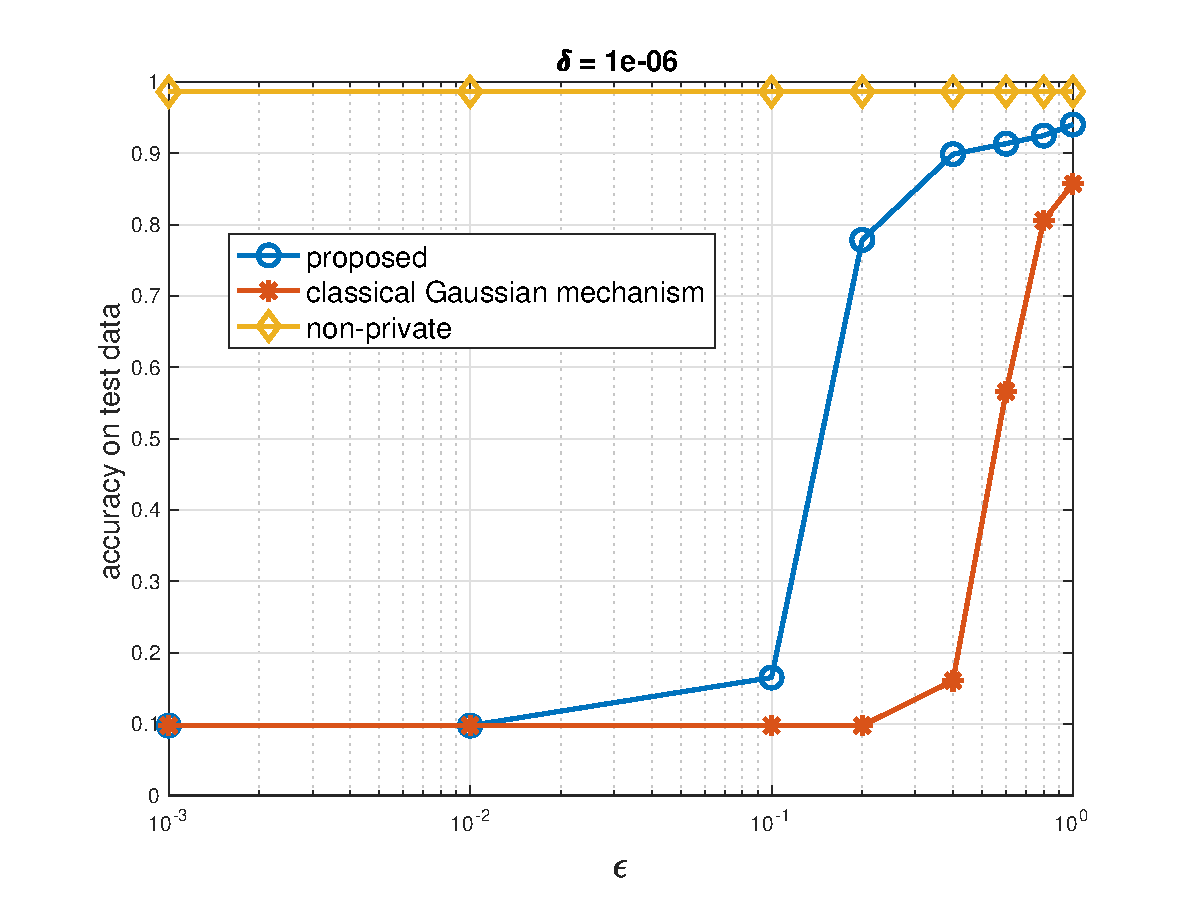
\includegraphics[width = 1.5in]{images/M_1}\label{fig_M_1}} \hfil \subfigure[$\delta = 1\mathrm{e}{-5}$.]{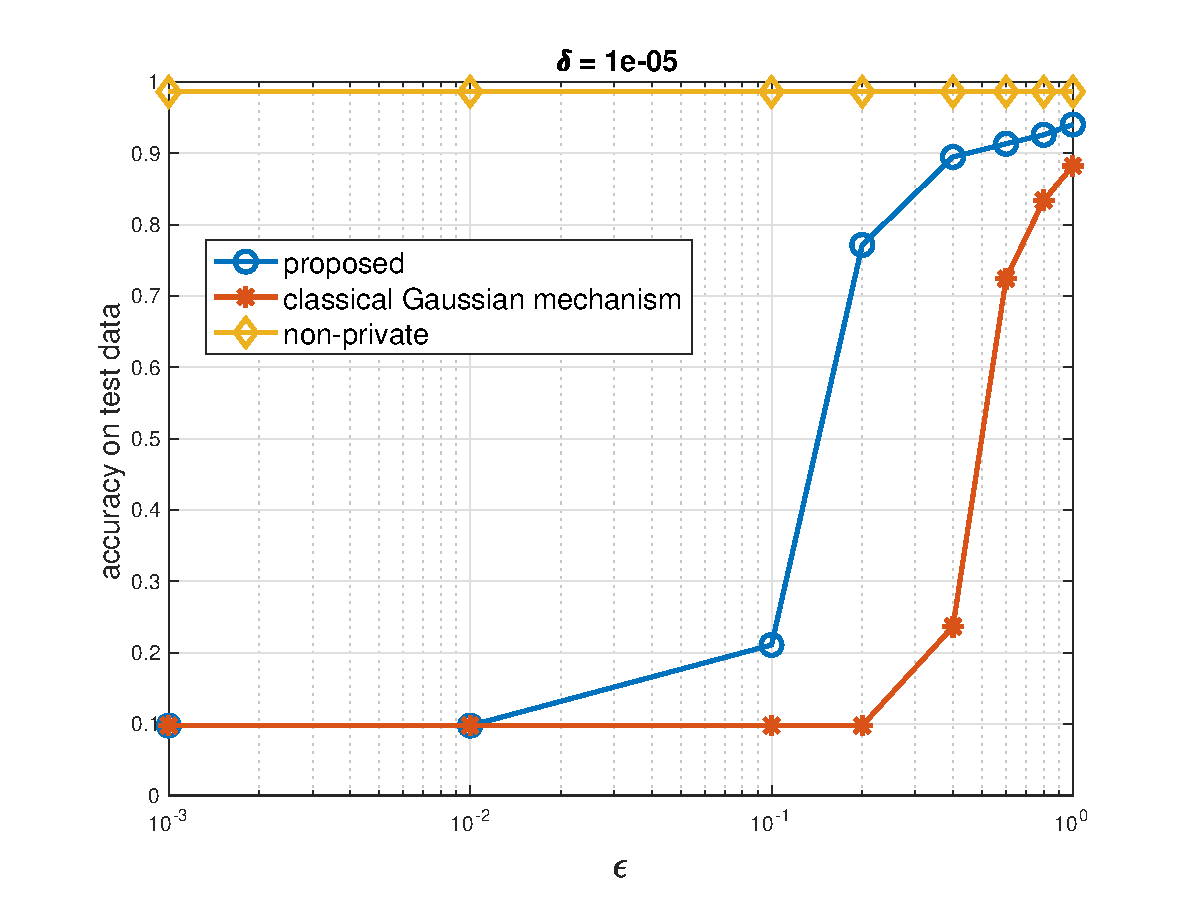
\includegraphics[width = 1.5in]{images/M_2}\label{fig_M_2}}}
% \centerline{ \subfigure[$\delta = 1\mathrm{e}{-4}$.]{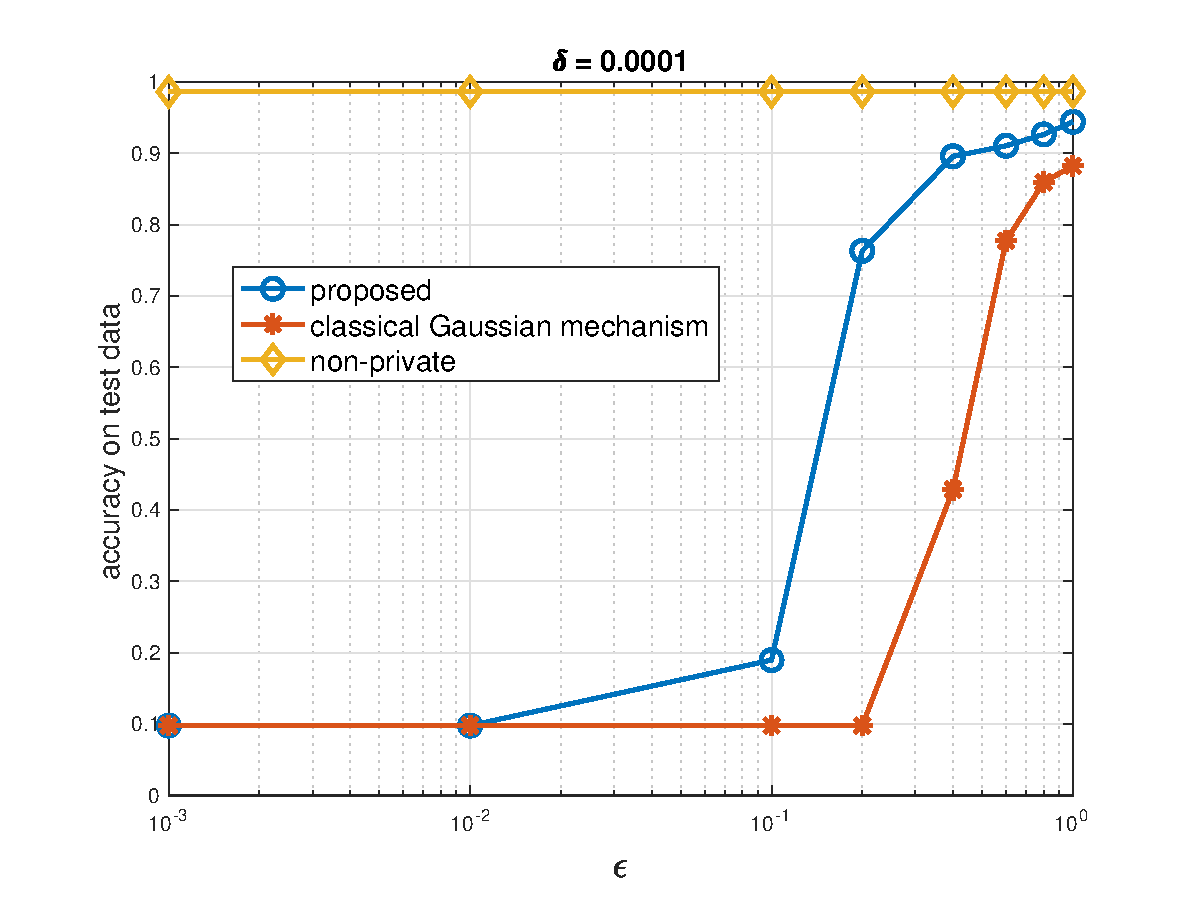
\includegraphics[width = 1.5in]{images/M_3}\label{fig_M_3}} \hfil \subfigure[$\delta = 1\mathrm{e}{-3}$.]{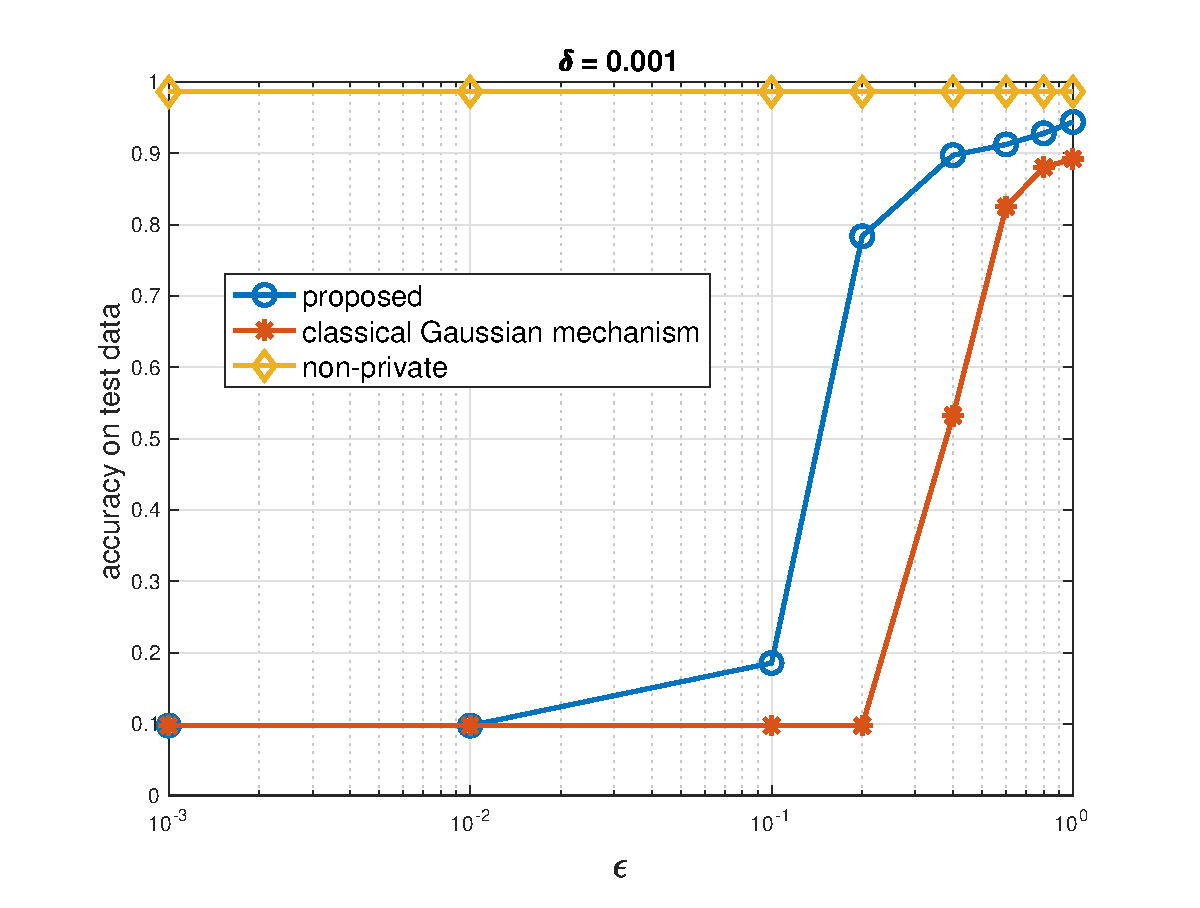
\includegraphics[width = 1.5in]{images/M_4}\label{fig_M_4}}}
% \centerline{ \subfigure[$\delta = 1\mathrm{e}{-2}$.]{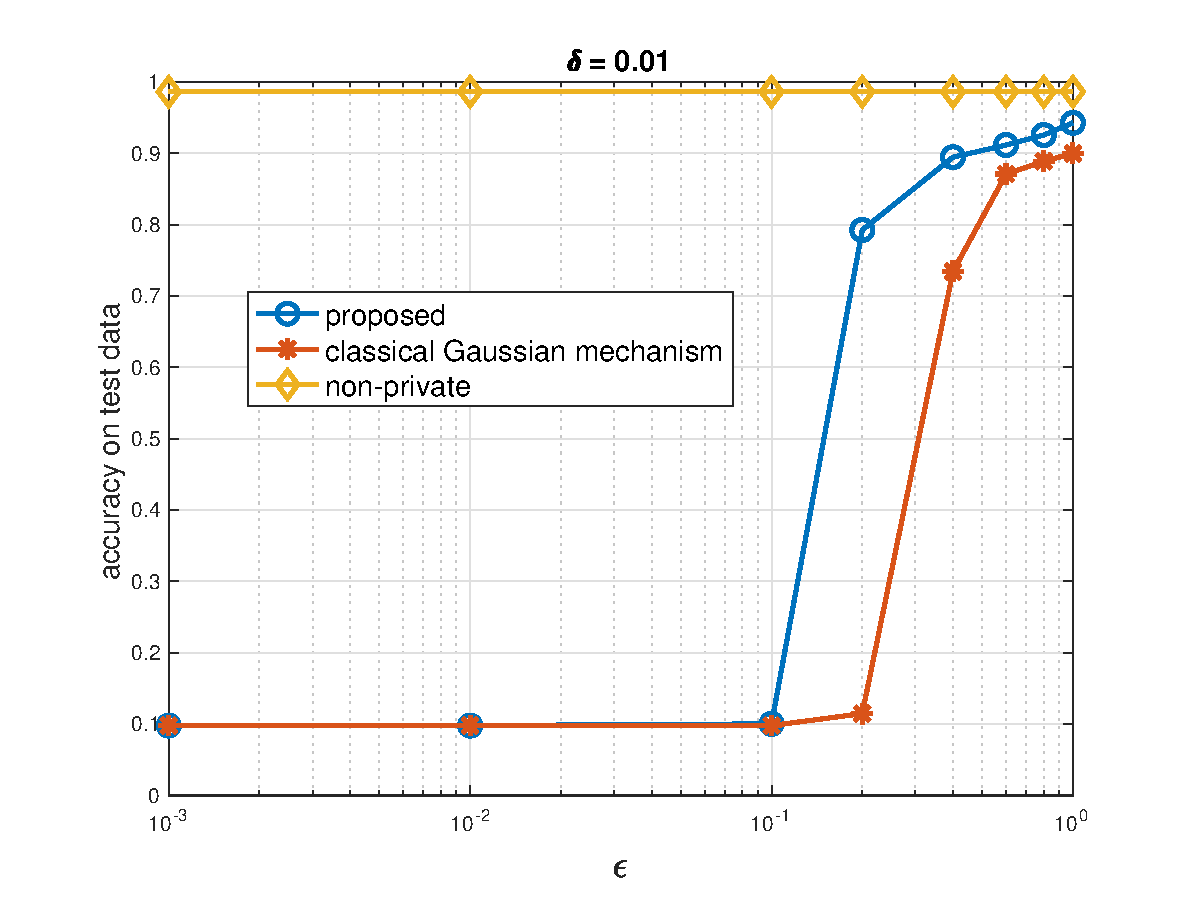
\includegraphics[width = 1.5in]{images/M_5}\label{fig_M_5}} \hfil \subfigure[$\delta = 1\mathrm{e}{-1}$.]{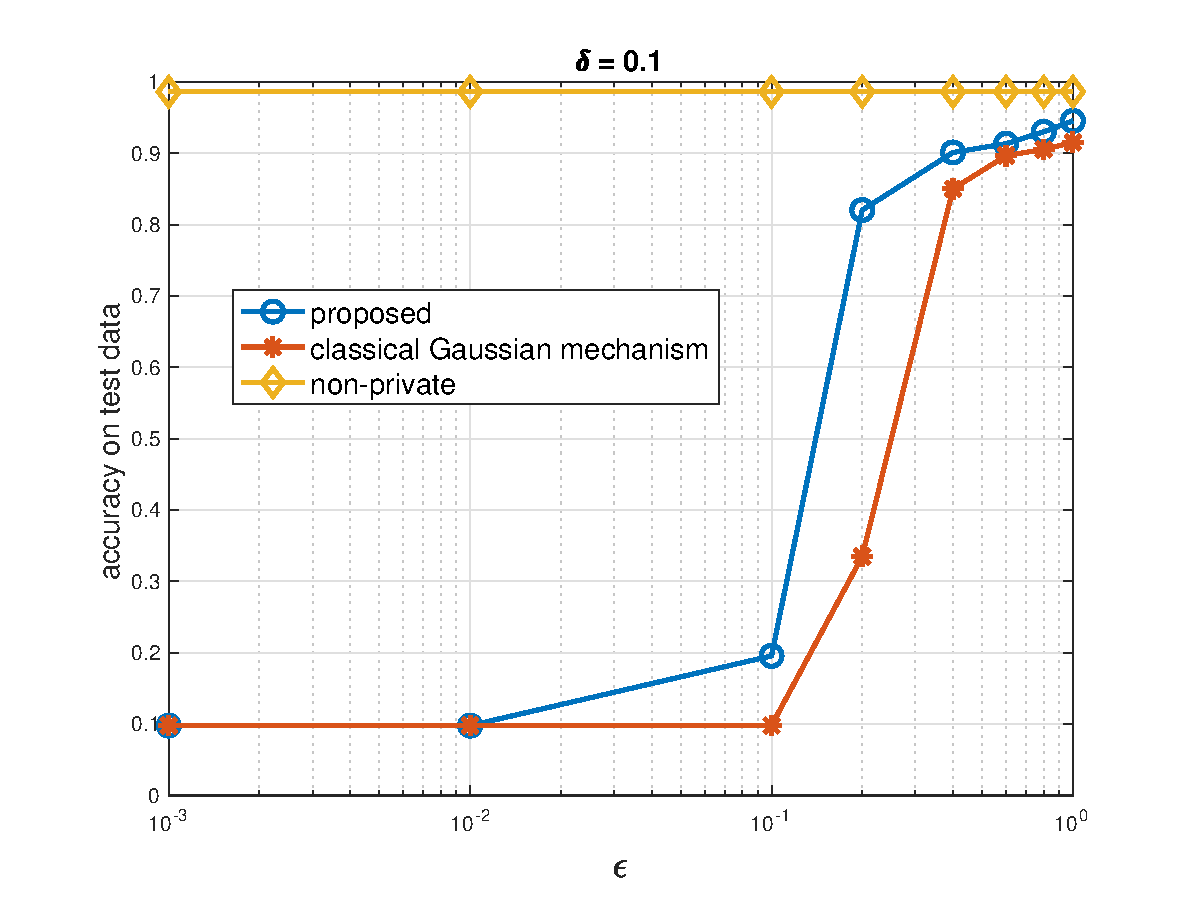
\includegraphics[width = 1.5in]{images/M_6}\label{fig_M_6}}}
% \centerline{ \subfigure[$\delta = 0.5$.]{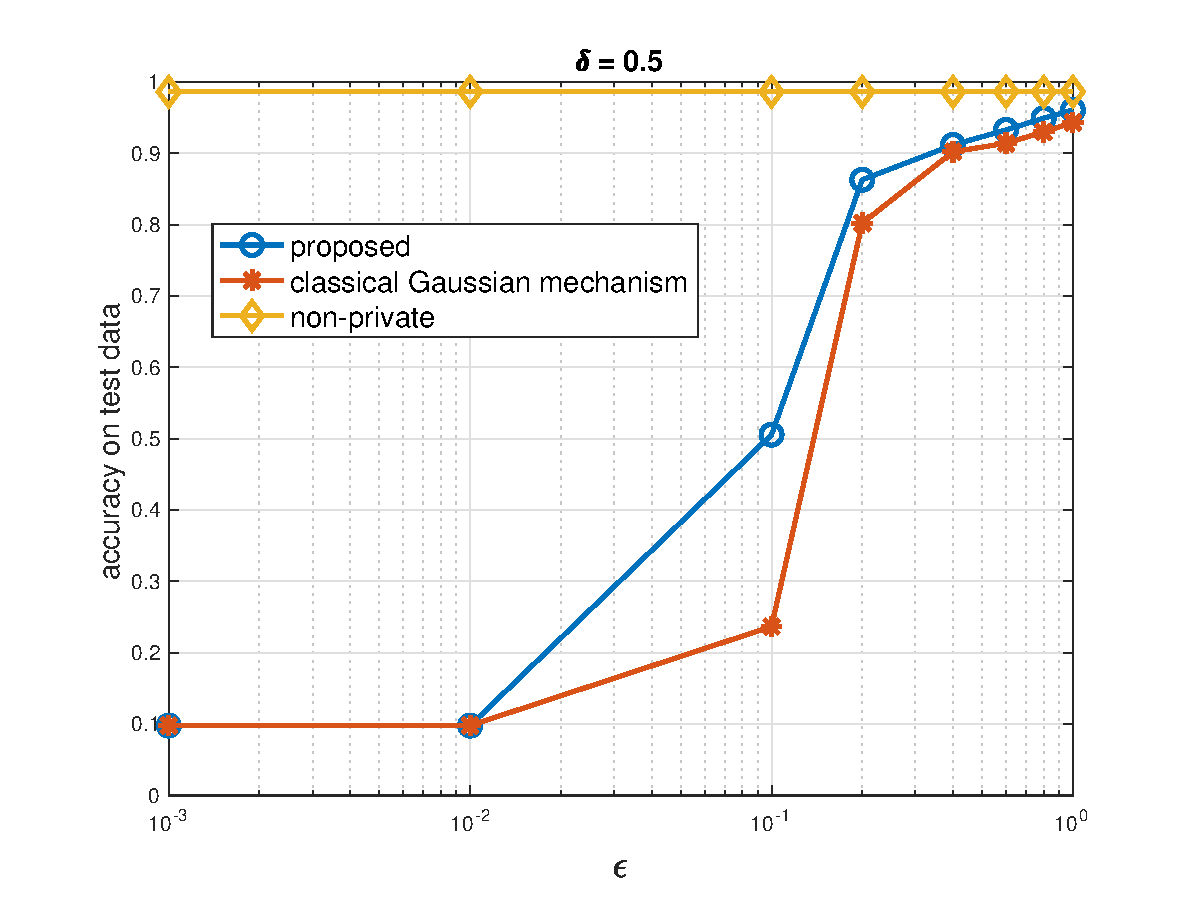
\includegraphics[width = 1.5in]{images/M_7}\label{fig_M_7}} \hfil \subfigure[$\delta = 0.9$.]{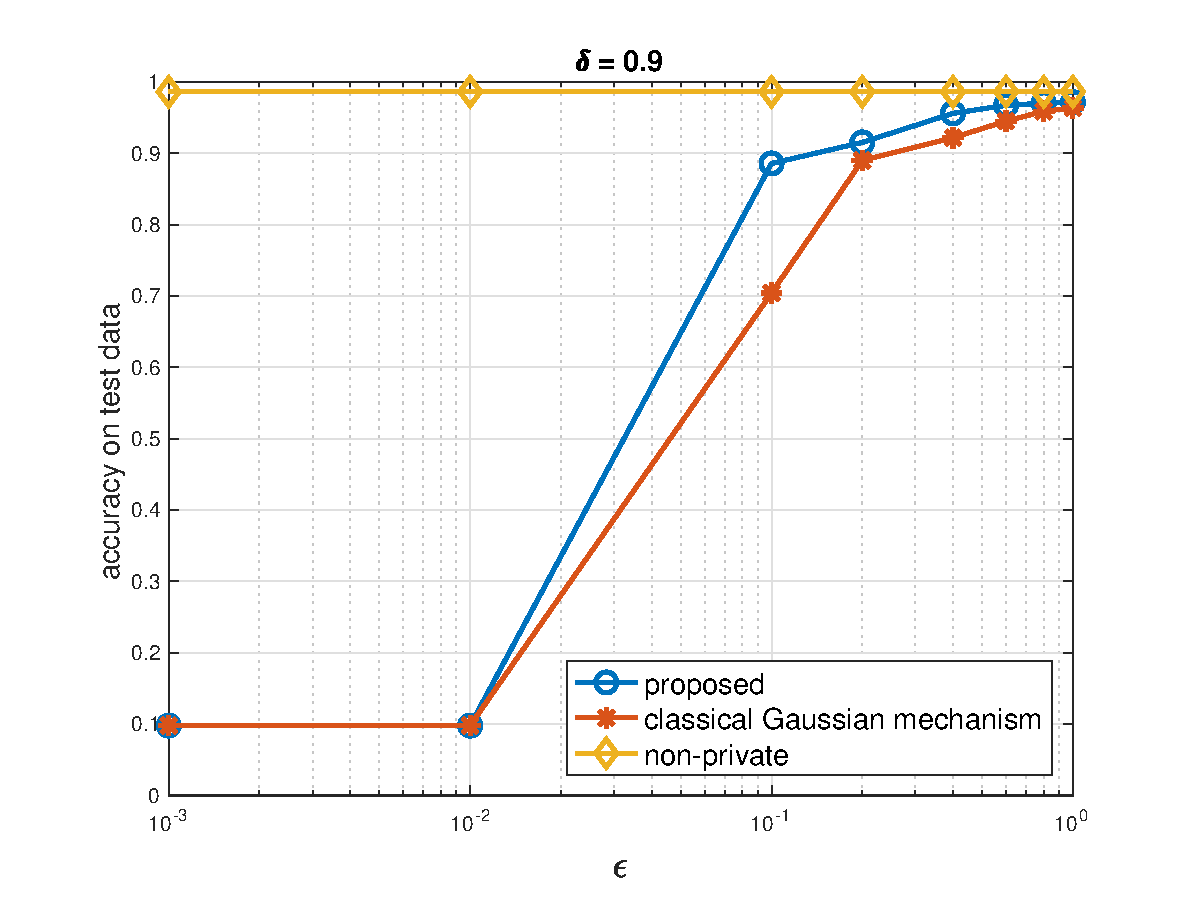
\includegraphics[width = 1.5in]{images/M_8}\label{fig_M_8}}}
% \caption{The effect of $\epsilon$ on MNIST test data classification accuracy.}\label{fig_M_first_part}
% \end{figure}
% \begin{figure}
% \centerline{ \subfigure[$\epsilon = 1\mathrm{e}{-3}$.]{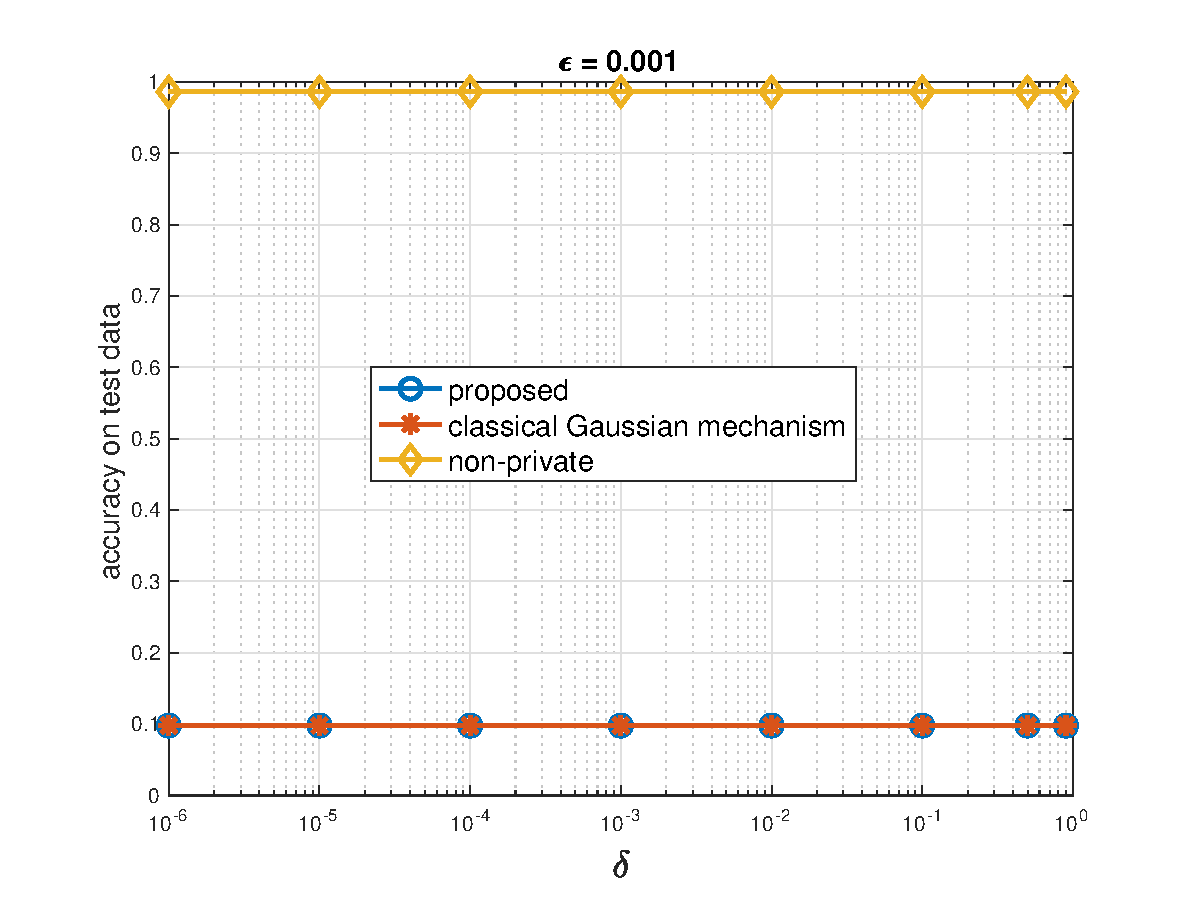
\includegraphics[width = 1.5in]{images/M_9}\label{fig_M_9}} \hfil \subfigure[$\epsilon = 1\mathrm{e}{-2}$.]{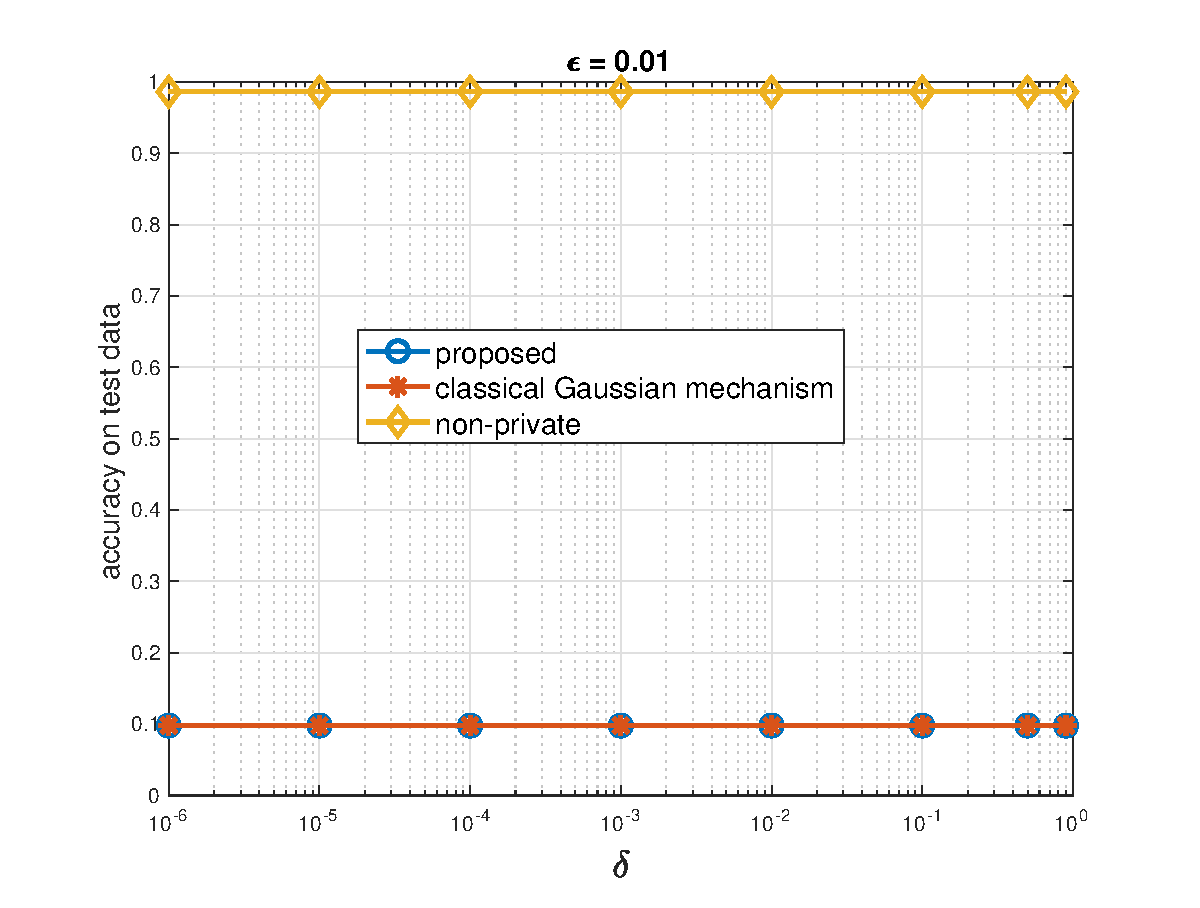
\includegraphics[width = 1.5in]{images/M_10}\label{fig_M_10}}}
% \centerline{ \subfigure[$\epsilon = 1e-1$.]{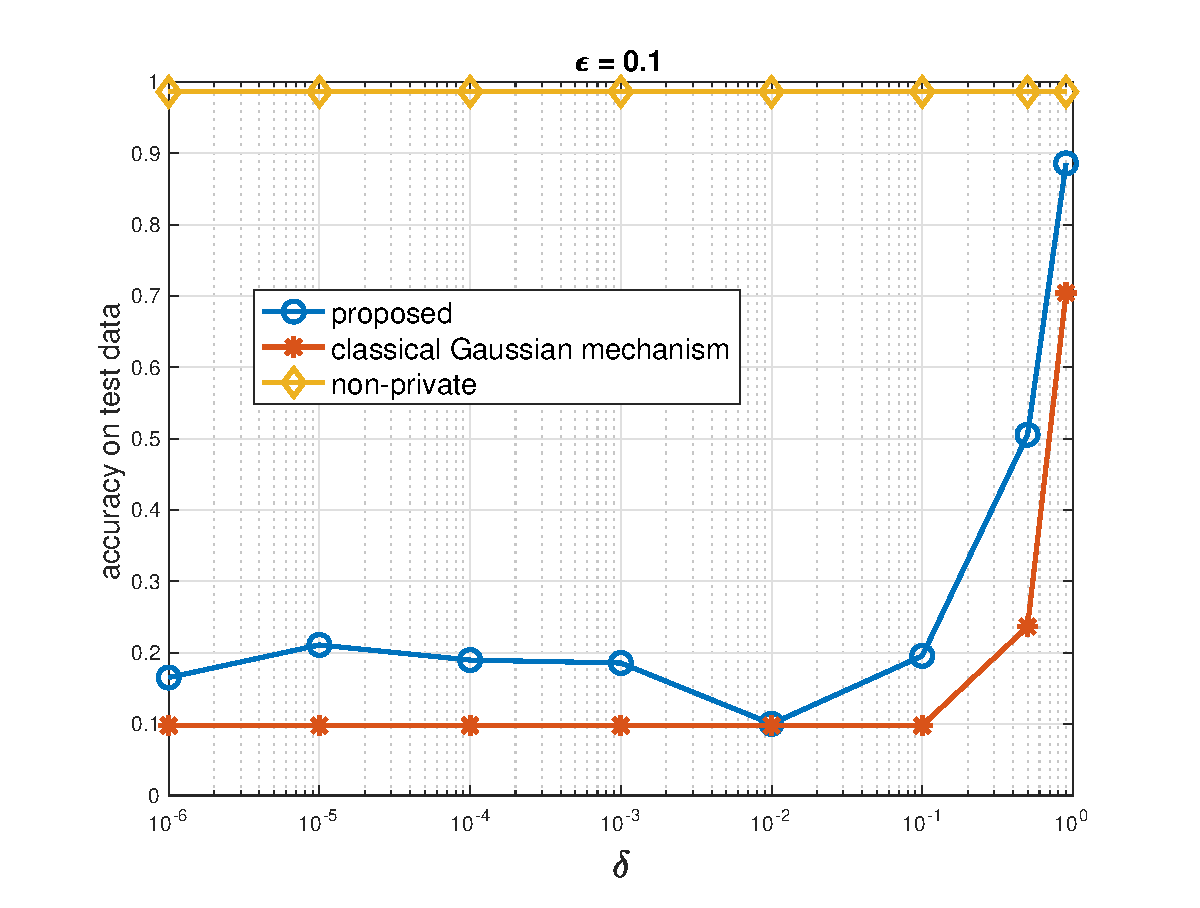
\includegraphics[width = 1.5in]{images/M_11}\label{fig_M_11}} \hfil \subfigure[$\epsilon = 0.2$.]{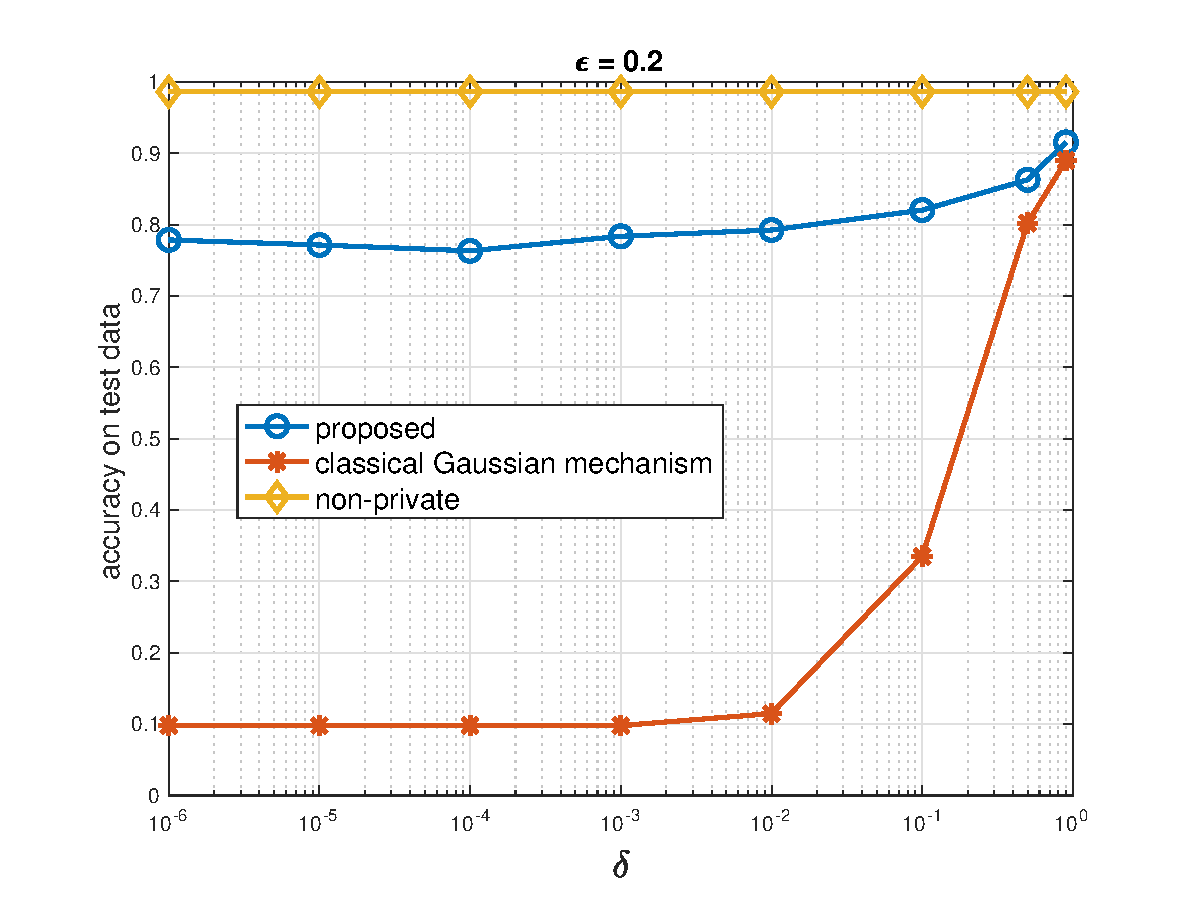
\includegraphics[width = 1.5in]{images/M_12}\label{fig_M_12}}}
% \centerline{ \subfigure[$\epsilon = 0.4$.]{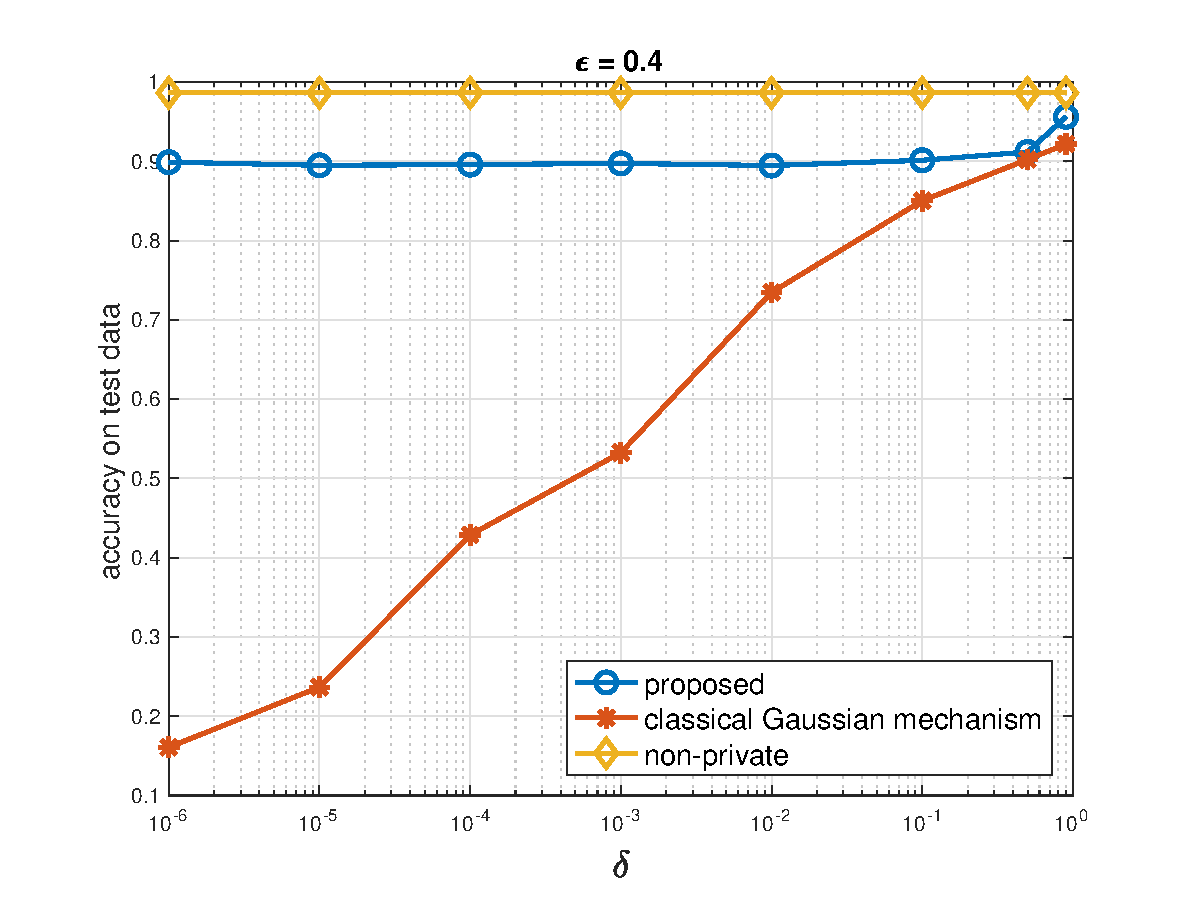
\includegraphics[width = 1.5in]{images/M_13}\label{fig_M_13}} \hfil \subfigure[$\epsilon = 0.6$.]{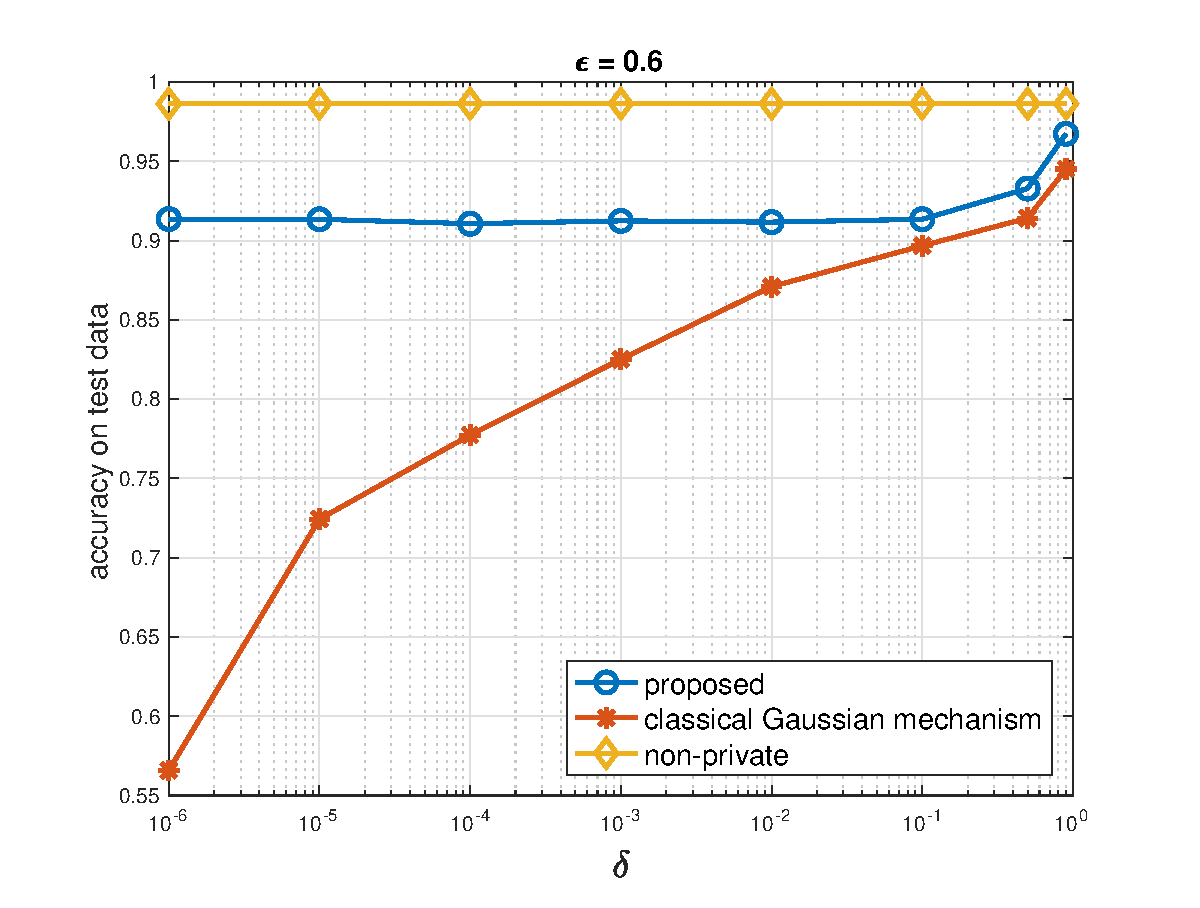
\includegraphics[width = 1.5in]{images/M_14}\label{fig_M_14}}}
% \centerline{ \subfigure[$\epsilon = 0.8$.]{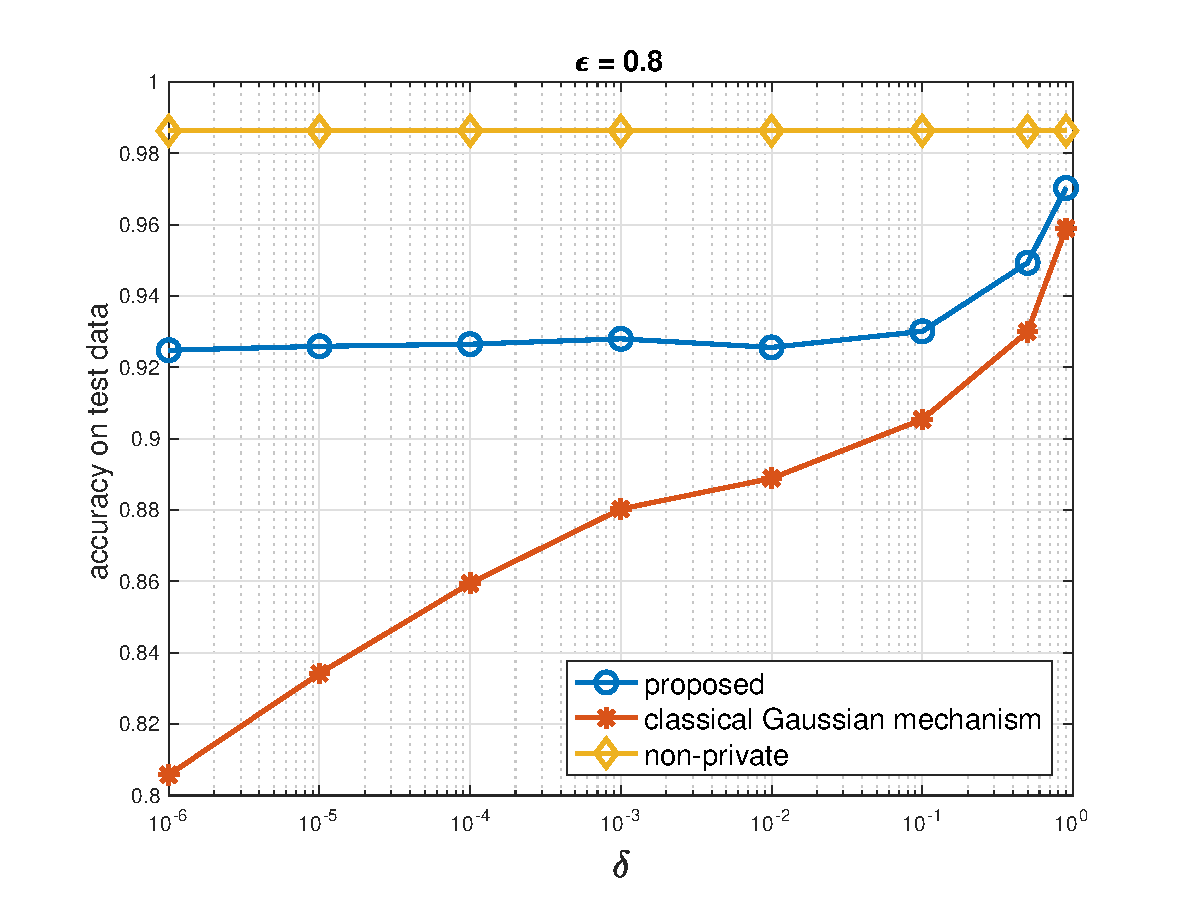
\includegraphics[width = 1.5in]{images/M_15}\label{fig_M_15}} \hfil \subfigure[$\epsilon = 1$.]{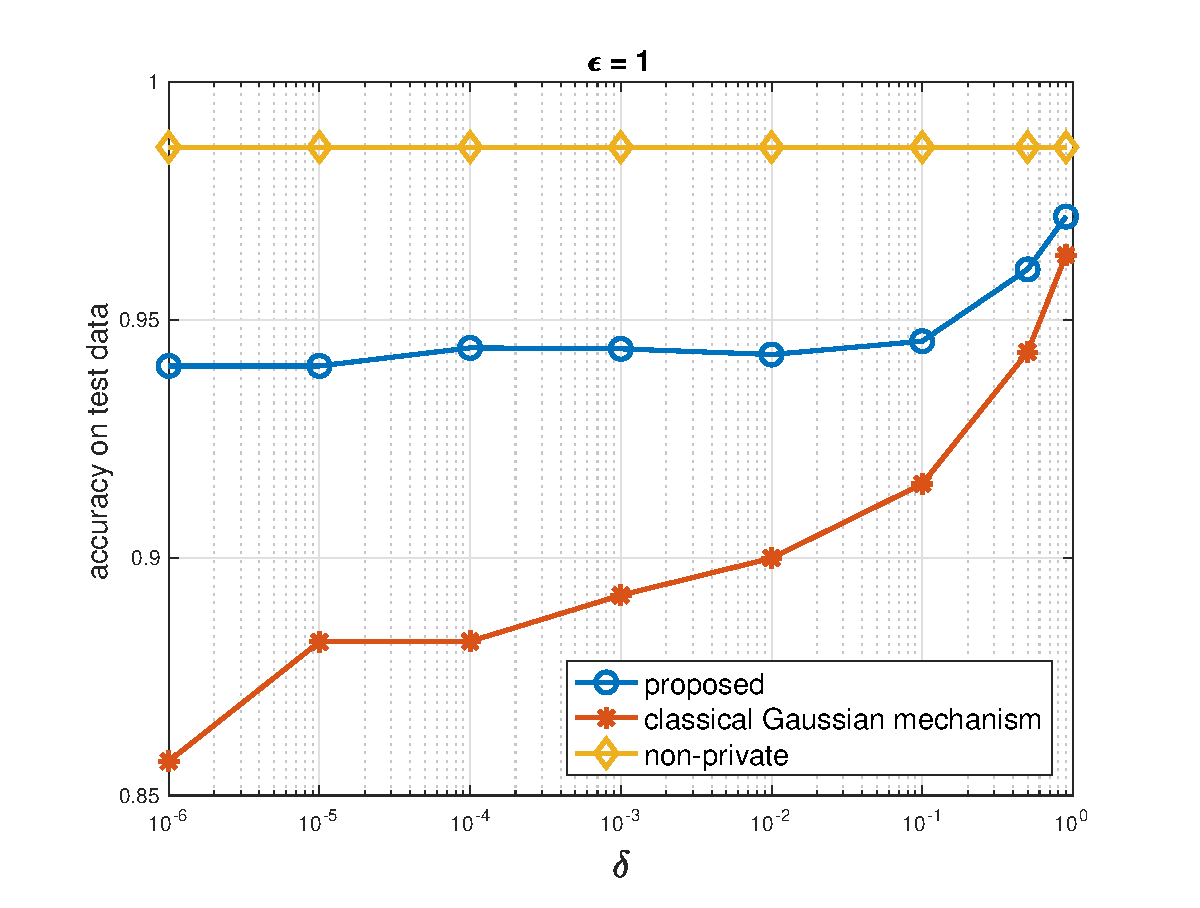
\includegraphics[width = 1.5in]{images/M_16}\label{fig_M_16}}}
% \caption{The effect of $\delta$ on MNIST test data classification accuracy.}\label{fig_M_second_part}
% \end{figure}

% Numerous experiments are made to study the effect of $\epsilon$ and $\delta$ on the accuracy in classifying test images. The non-private version of the proposed method is applied to calculate the reference performance of the method. The experimental results have been displayed in Fig.~\ref{fig_M_first_part} and Fig.~\ref{fig_M_second_part}. The following inferences are drawn from the results: 1) The proposed method consistently achieves a higher accuracy than the classical Gaussian mechanism. This is observed in all subfigures of Fig.~\ref{fig_M_first_part} and Fig.~\ref{fig_M_second_part} except in Fig.~\ref{fig_M_9} and Fig.~\ref{fig_M_10} where both mechanisms perform nearly the same. 2) In very-high privacy regime (i.e. when $\epsilon \leq 1\mathrm{e}{-2}$ for this particular dataset), the noise level is so high that the optimality of the proposed mechanism doesn't manifest itself to any observed gain in the accuracy. This should explain the nearly same performance of both mechanism in Fig.~\ref{fig_M_9} and Fig.~\ref{fig_M_10}. 

% To study the robustness, the test images are contaminated by zero-mean Gaussian additive noise with varying level of standard deviation. The widely used Convolutional Neural Network (CNN) is taken as a reference for comparing the performance. A CNN with the patch size of $5 \times 5$, first convolutional layer of 32 features, second convolutional layer of 64 features, and densely connected layer of 1024 neurons is considered. The convolutions use a stride of one and are zero padded. The pooling is max pooling over $2\times2$ blocks. The CNN was trained for 10000 iterations where each iteration uses a batch size of 100 images. 
% \begin{table}
% \renewcommand{\arraystretch}{1.3}
% \caption{The effect of noise level on the performance in classifying MNIST digits}
% \label{table_robustness_results} \centering
% \begin{tabular}{c||*{2}{c}}
% \hline
% \bfseries $\begin{array}{c} \mbox{noise} \\ \mbox{standard deviation} \end{array}$ & \multicolumn{2}{c}{\bfseries classification accuracy on test images}  \\
% \cline{2-3} 
%  & \bfseries proposed  &    \bfseries CNN  \\ 
% \hline \hline  
% 0 & 0.9863    & \textbf{0.9897}  \\
% 0.2 &   \textbf{0.9825}   & 0.9608  \\ 
% 0.4 & \textbf{0.9630}  & 0.8198 \\ 
% 0.6 & \textbf{0.9019}   & 0.6227  \\ 
% 0.8 & \textbf{0.7818}  & 0.4482  \\
% 1 & \textbf{0.6335}  & 0.3203 \\
% \hline \hline
% \end{tabular}
% \end{table} 

% Table~\ref{table_robustness_results} lists the performance of non-private version of the proposed method. The robustness of the proposed approach is clearly observed in Table~\ref{table_robustness_results} as with an increasing level of noise the decrease in classification accuracy is observed to be much slower in the case of proposed method than CNN. 

% \subsubsection{Freiburg Groceries Dataset}
% The image category classification problem is considered using ``Freiburg Groceries Dataset''~\cite{DBLP:journals/corr/JundAEB16} to study the privacy of the proposed method and to compare it with the classical machine learning algorithms. The dataset~\cite{DBLP:journals/corr/JundAEB16} contains around 5000 labeled images of grocery products commonly sold in Germany. The images have been categorized into 25 different classes of grocery products. A feature vector is created from each image by extracting features from ``AlexNet'' and ``VGG-16'' networks which are pre-trained Convolutional Neural Networks. The activations of the fully connected layer ``fc6'' in AlexNet constitute a $4096-$dimensional feature vector. Similarly, the activations of the fully connected layer ``fc6'' in VGG-16 constitute another $4096-$dimensional feature vector. The features extracted by both networks are joined together to form a $8192-$dimensional vector. The complete set of feature vectors is normalized to have zero-mean and unity-variance along each dimension.  

% We choose a training-testing data split and a distributed learning scenario was created assuming that a class's complete training data is owned by a single participant. Thus the number of participants is equal to the number of classes. Several experiments have been made to study the method's $(\epsilon,\delta)-$differential privacy against perturbation (in one element of data vector), with perturbation magnitude upper bounded by $d = 0.1$. Also, the non-private version of our method is compared with the following machine learning techniques: 1) $k$-nearest neighbor ($k$-NN) with $k = 1$; 2) Naive Bayes; 3) Decision Tree; 4) Support Vector Machine (SVM); 5) Ensemble Learning via Boosting 100 Classification Trees; 6) Random Forest of 100 Classification Trees. 

% Table~\ref{table_results_grocery_images}, Fig.~\ref{fig_G_first_part}, and Fig.~\ref{fig_G_second_part} state the experimental results. The following inferences are drawn from the obtained results: 1) A higher accuracy of the proposed method in comparison to Gaussian mechanism is consistently observed in all subfigures of Fig.~\ref{fig_G_first_part} and Fig.~\ref{fig_G_second_part} except in Fig.~\ref{fig_G_9} where both mechanisms perform nearly same. 2) In very-high privacy regime (i.e. when $\epsilon \leq 1\mathrm{e}{-3}$ for this particular dataset), the noise level is so high that the optimality of the proposed mechanism doesn't manifest itself to any observed gain in the accuracy. This should explain the nearly same performance of both mechanism in Fig.~\ref{fig_G_9}. 3) Also in very-low privacy regime, e.g. in Fig.~\ref{fig_G_16} at higher $\delta$ values, the noise level is so low that the both mechanism perform nearly the same. 4) A better performance of the proposed fuzzy based method in comparison to classical machine learning methods is observed (in Table~\ref{table_results_grocery_images}) in classifying high-dimensional data vectors. 
% \begin{table}
% \renewcommand{\arraystretch}{1.3}
% \caption{Results of experiments on Freiburg groceries dataset}
% \label{table_results_grocery_images} \centering
% \begin{tabular}{c||c}
% \hline
% \bfseries method  & \bfseries testing accuracy in \%   \\
% \hline \hline  
% $(0.1,1\mathrm{e}{-6})-$differentially private proposed & \textbf{78.88} \\
% $(0.1,1\mathrm{e}{-6})-$differentially private Gaussian & 42.53 \\
% Non-private proposed &  \textbf{88.50} \\
% Non-private $1$-NN & 78.00      \\
% Non-private SVM & 77.90      \\
% Non-private Random Forest &  63.17   \\
% Non-private Naive Bayes & 56.78    \\
% Non-private Ensemble Learning & 38.31     \\
% Non-private Decision Tree & 31.34   \\
% \hline \hline
% \end{tabular}
% \end{table} 
% \begin{figure}[!h]
% \centerline{ \subfigure[$\delta = 1\mathrm{e}{-6}$.]{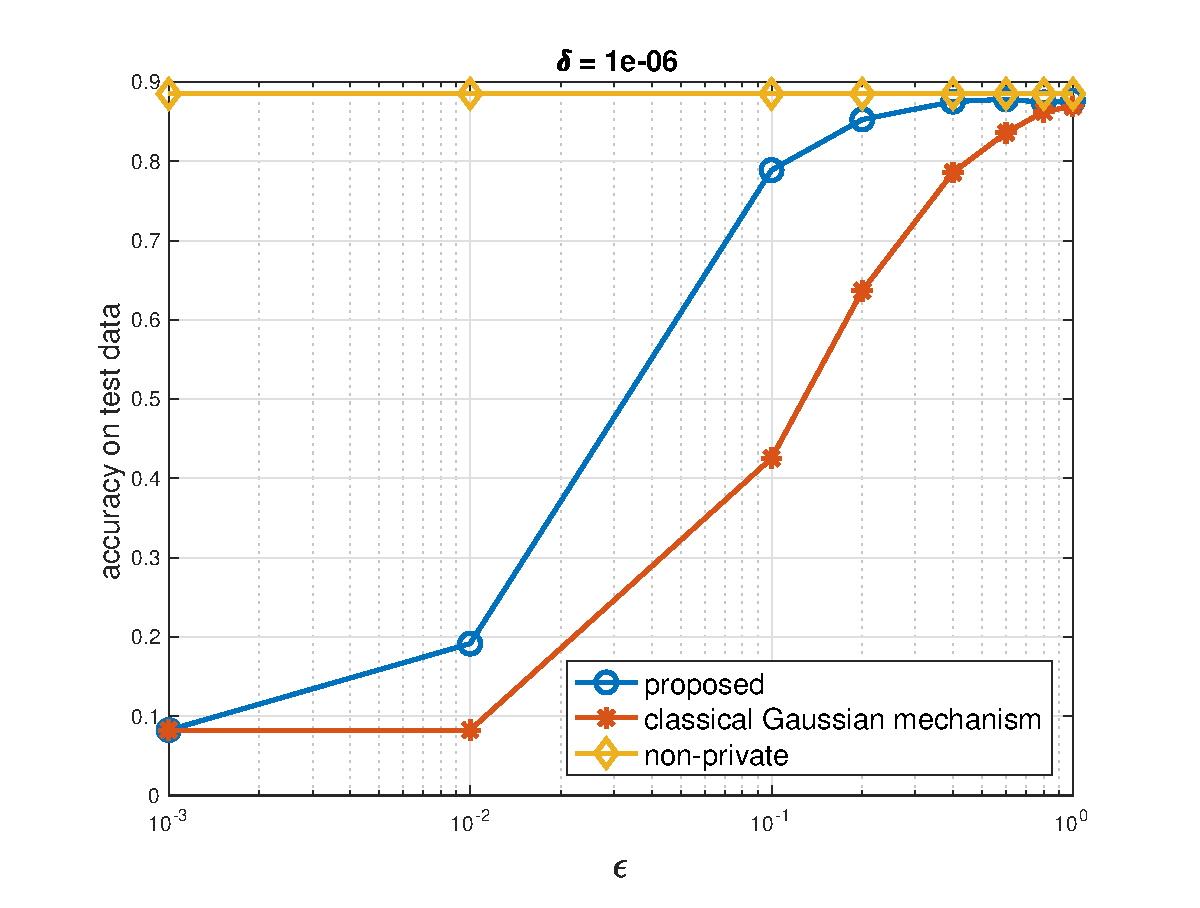
\includegraphics[width = 1.5in]{images/G_1}\label{fig_G_1}} \hfil \subfigure[$\delta = 1\mathrm{e}{-5}$.]{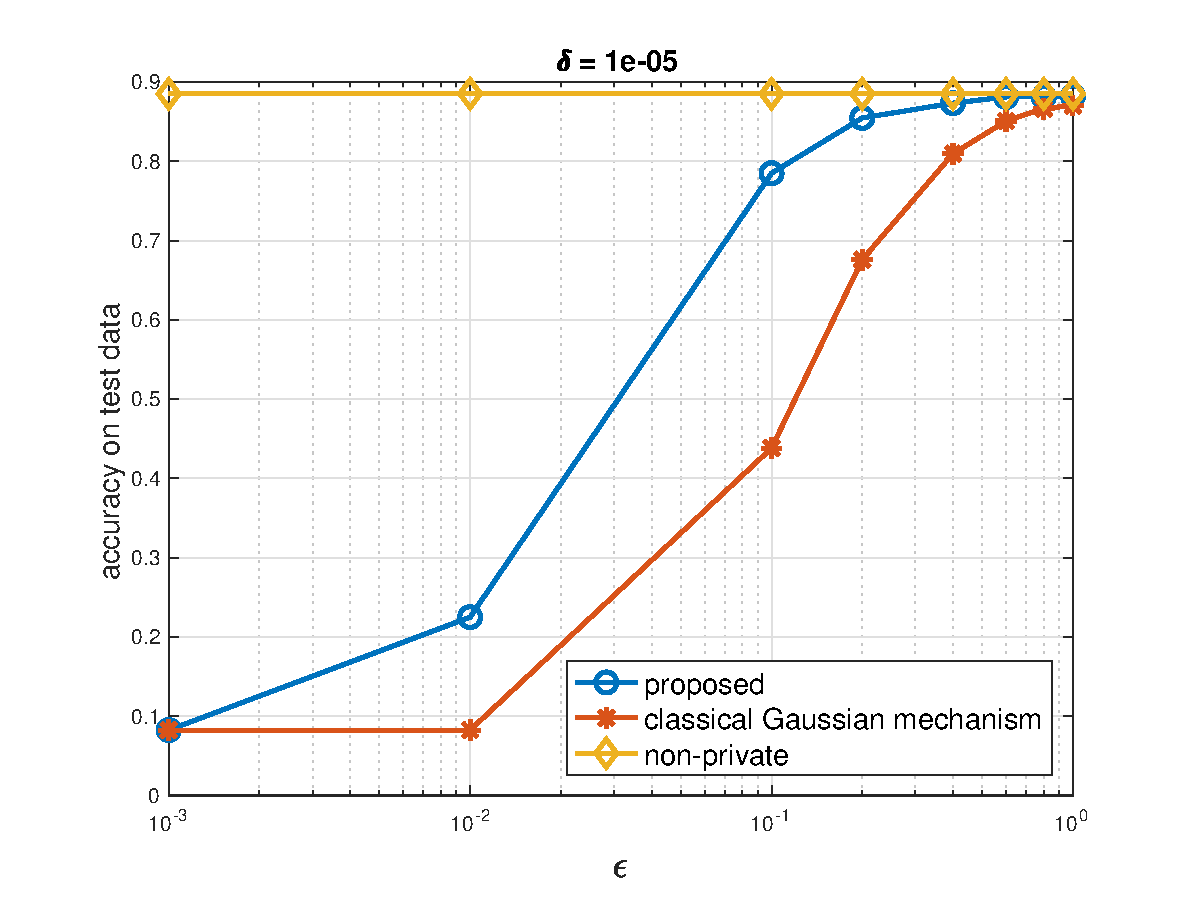
\includegraphics[width = 1.5in]{images/G_2}\label{fig_G_2}}}
% \centerline{ \subfigure[$\delta = 1\mathrm{e}{-4}$.]{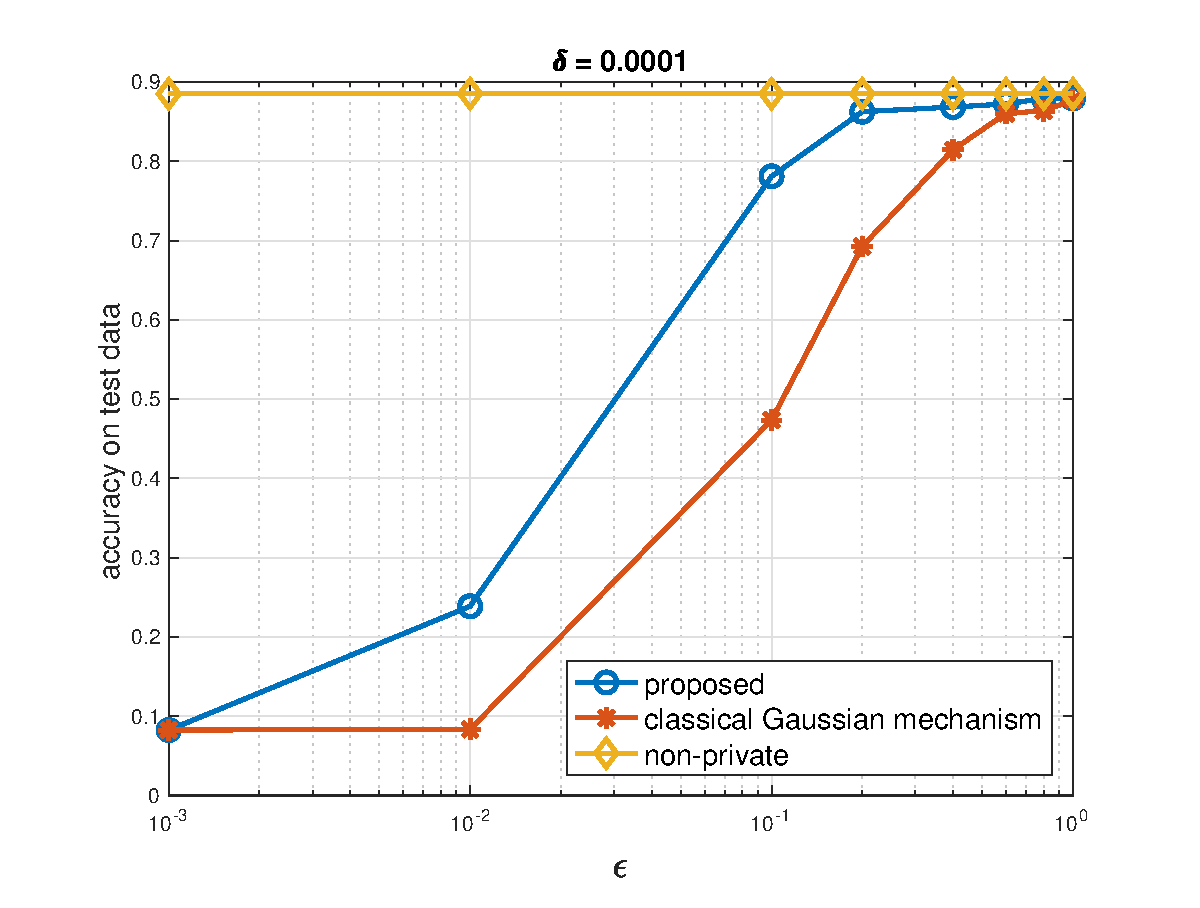
\includegraphics[width = 1.5in]{images/G_3}\label{fig_G_3}} \hfil \subfigure[$\delta = 1\mathrm{e}{-3}$.]{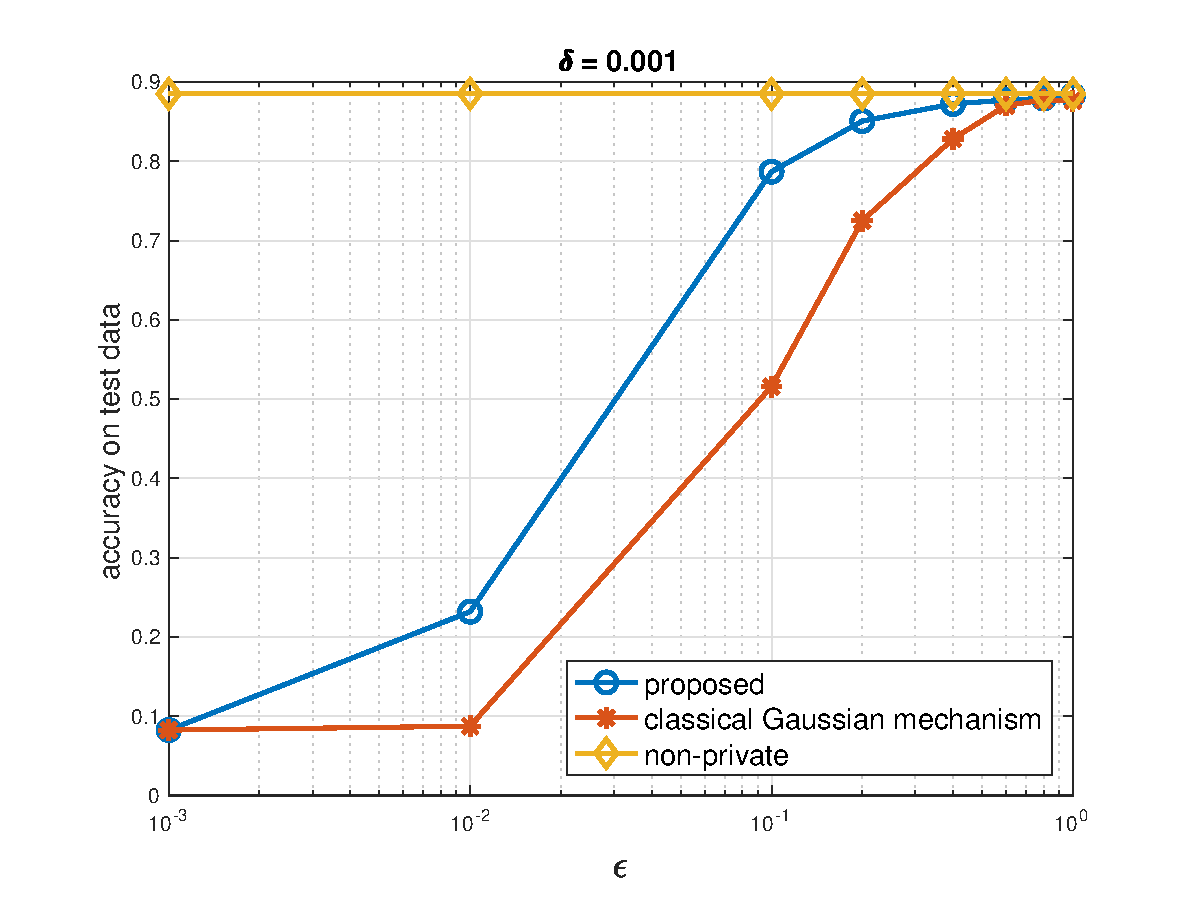
\includegraphics[width = 1.5in]{images/G_4}\label{fig_G_4}}}
% \centerline{ \subfigure[$\delta = 1\mathrm{e}{-2}$.]{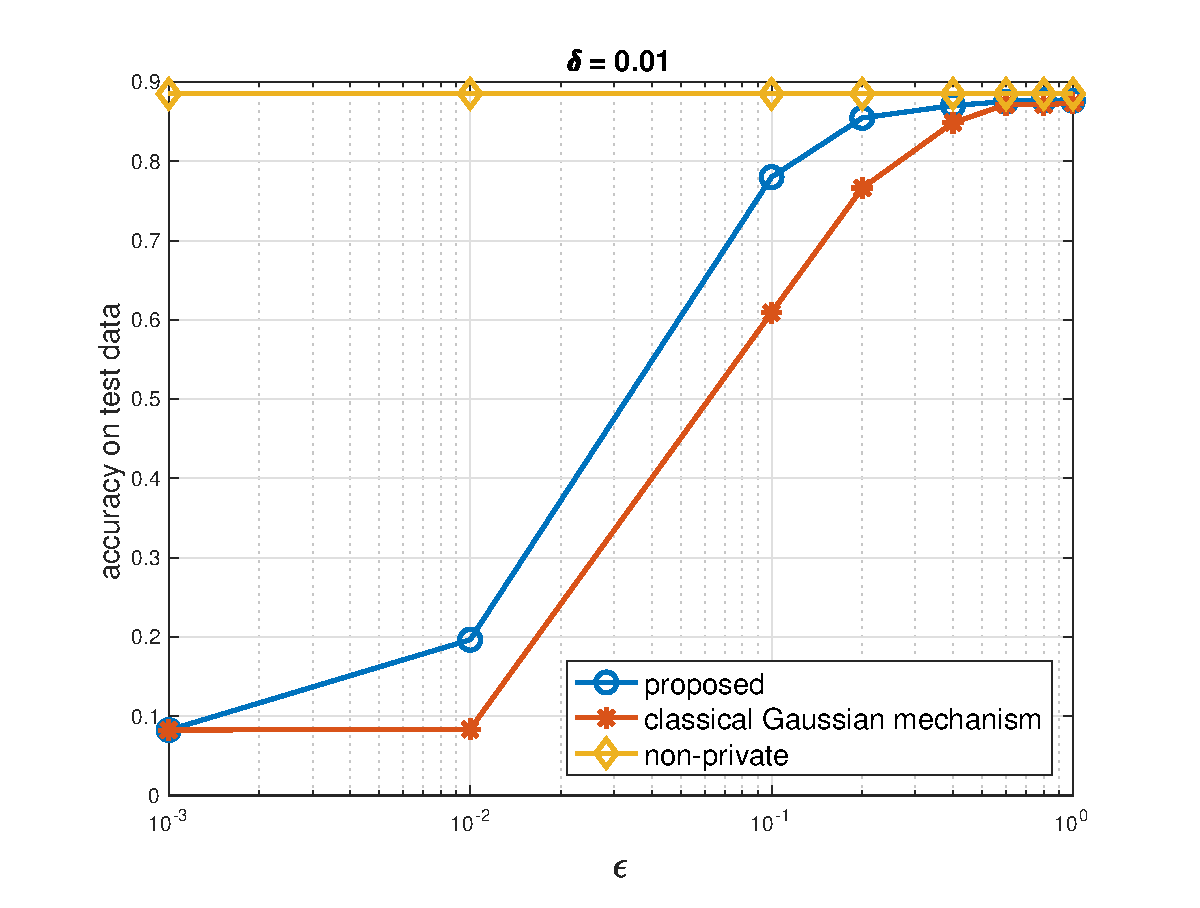
\includegraphics[width = 1.5in]{images/G_5}\label{fig_G_5}} \hfil \subfigure[$\delta = 1\mathrm{e}{-1}$.]{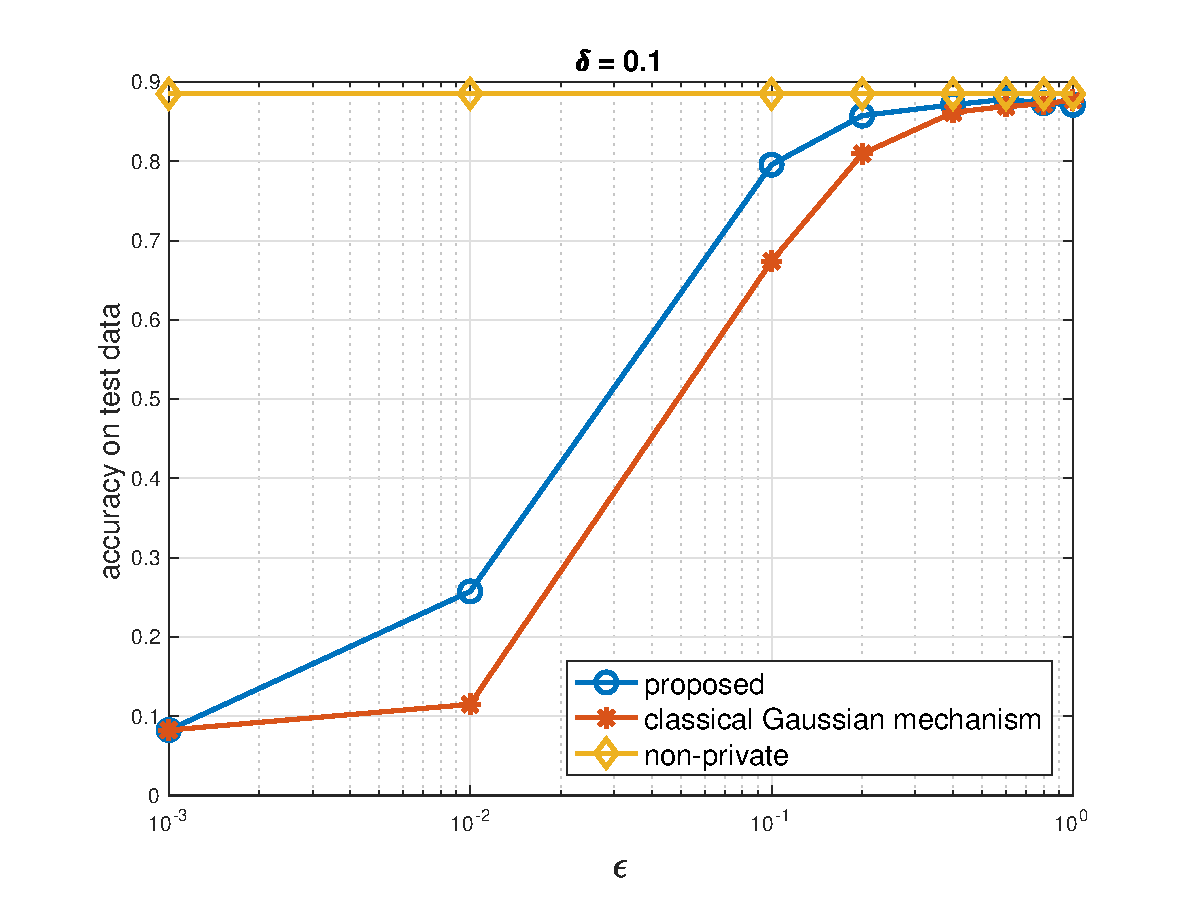
\includegraphics[width = 1.5in]{images/G_6}\label{fig_G_6}}}
% \centerline{ \subfigure[$\delta = 0.5$.]{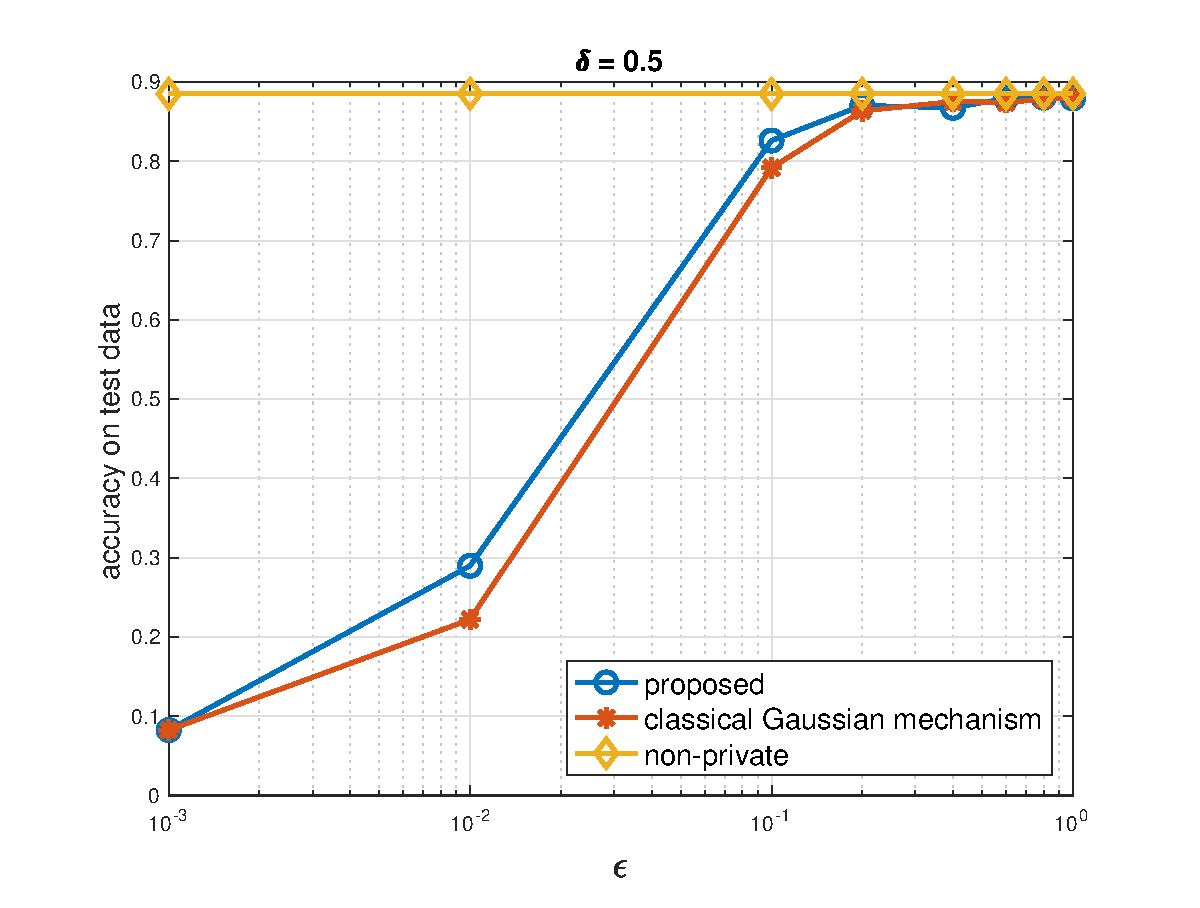
\includegraphics[width = 1.5in]{images/G_7}\label{fig_G_7}} \hfil \subfigure[$\delta = 0.9$.]{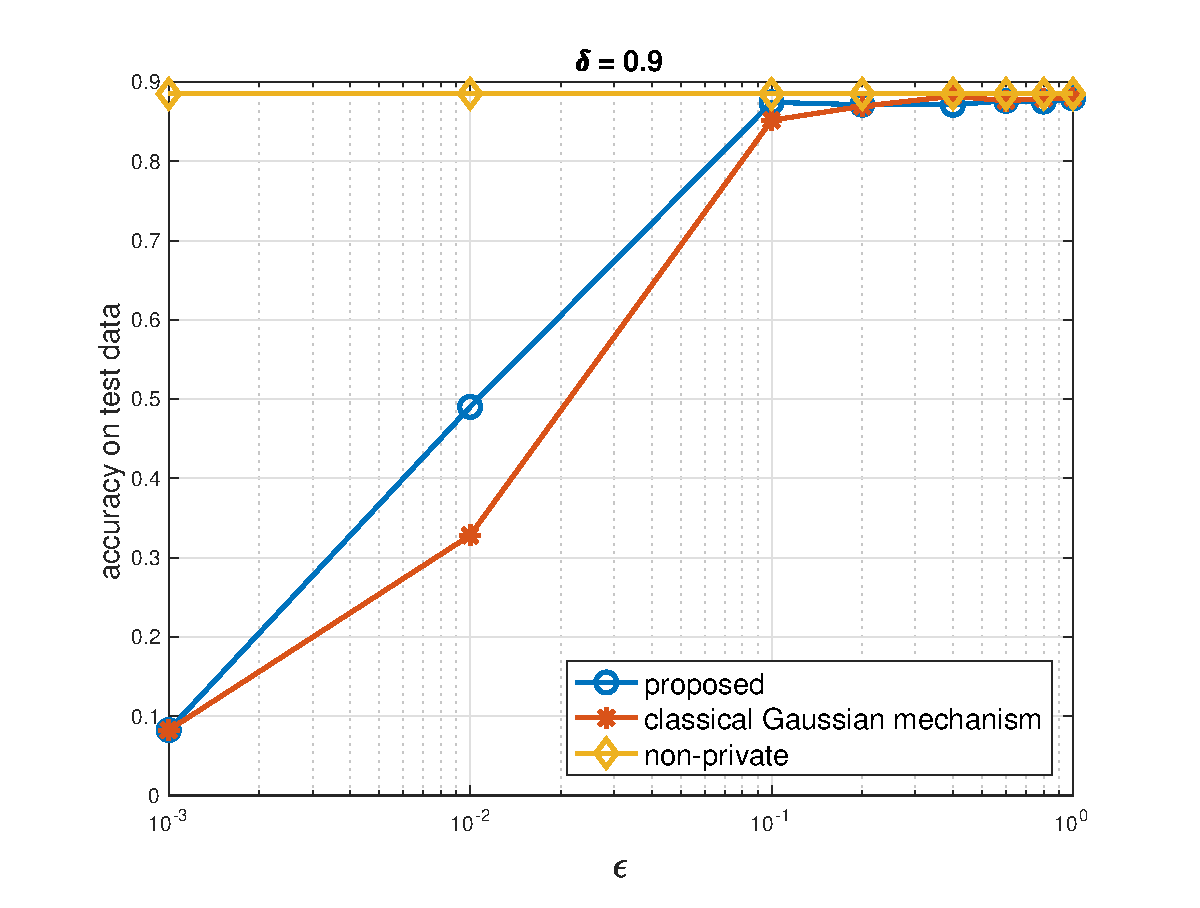
\includegraphics[width = 1.5in]{images/G_8}\label{fig_G_8}}}
% \caption{The effect of $\epsilon$ on Freiburg test data classification accuracy.}\label{fig_G_first_part}
% \end{figure}     
% \begin{figure}
% \centerline{ \subfigure[$\epsilon = 1\mathrm{e}{-3}$.]{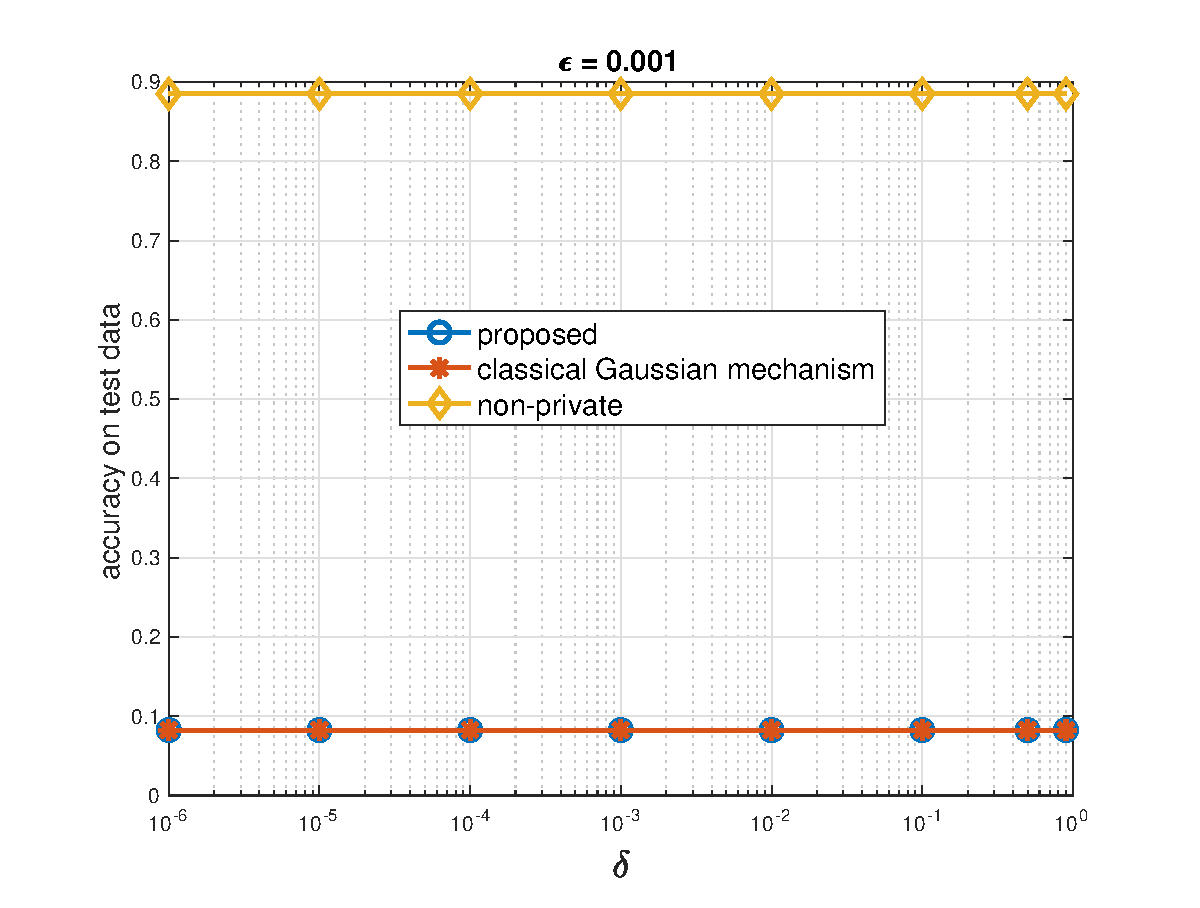
\includegraphics[width = 1.5in]{images/G_9}\label{fig_G_9}} \hfil \subfigure[$\epsilon = 1\mathrm{e}{-2}$.]{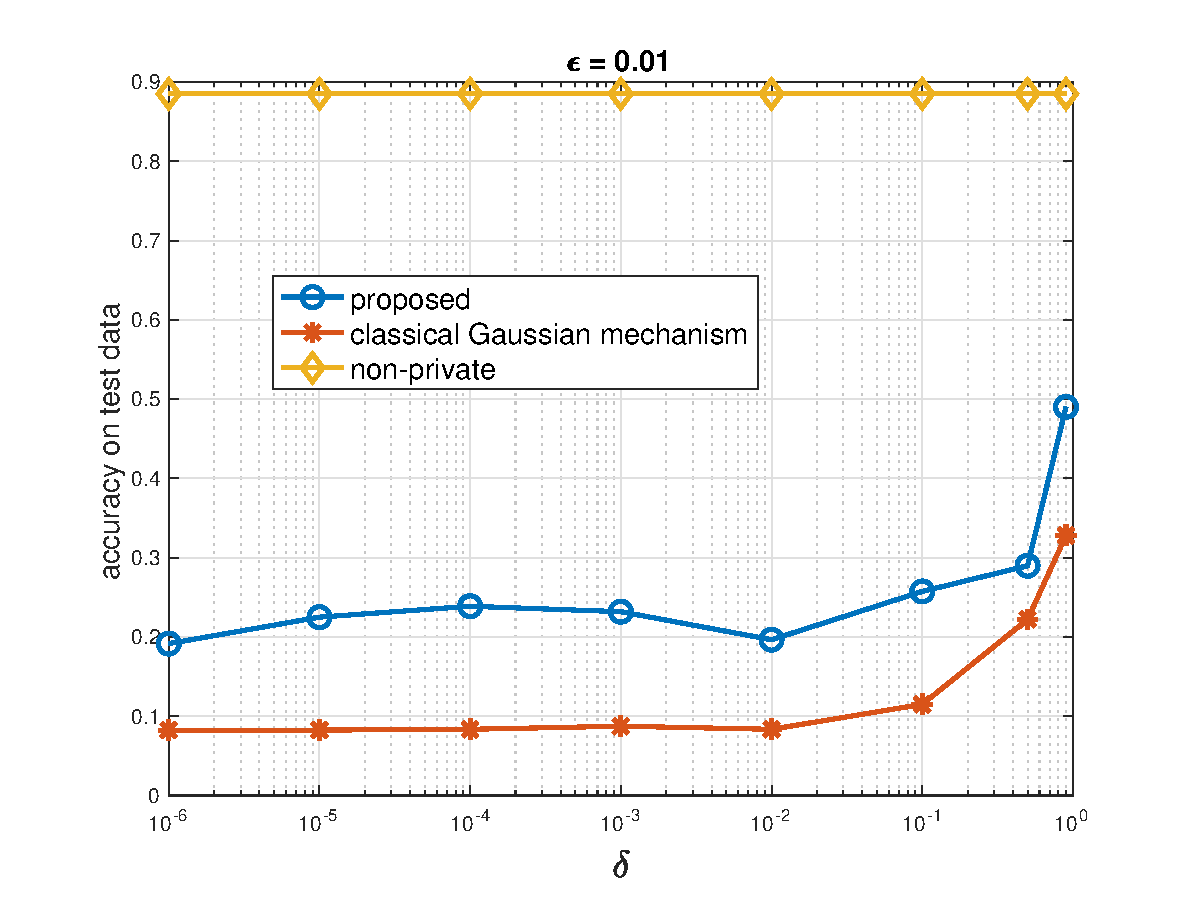
\includegraphics[width = 1.5in]{images/G_10}\label{fig_G_10}}}
% \centerline{ \subfigure[$\epsilon = 1\mathrm{e}{-1}$.]{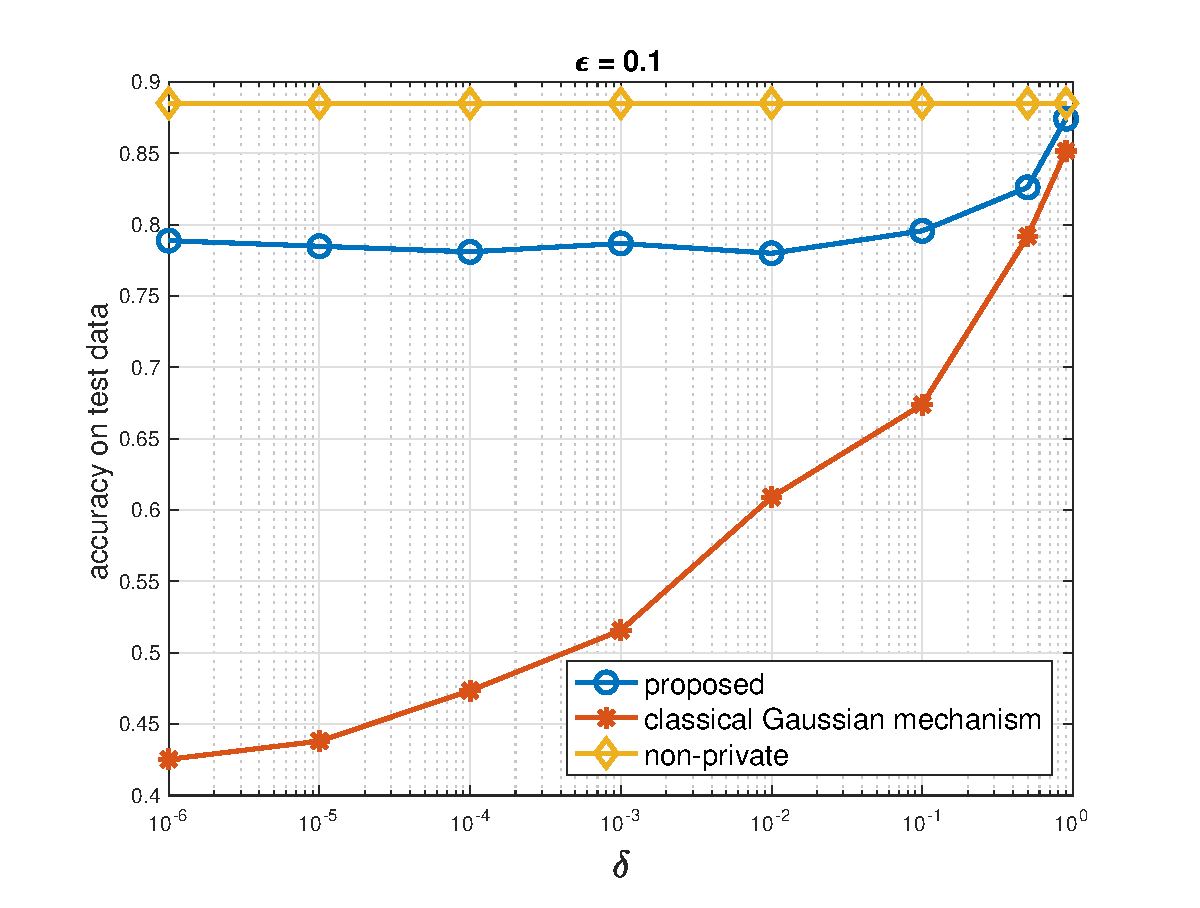
\includegraphics[width = 1.5in]{images/G_11}\label{fig_G_11}} \hfil \subfigure[$\epsilon = 0.2$.]{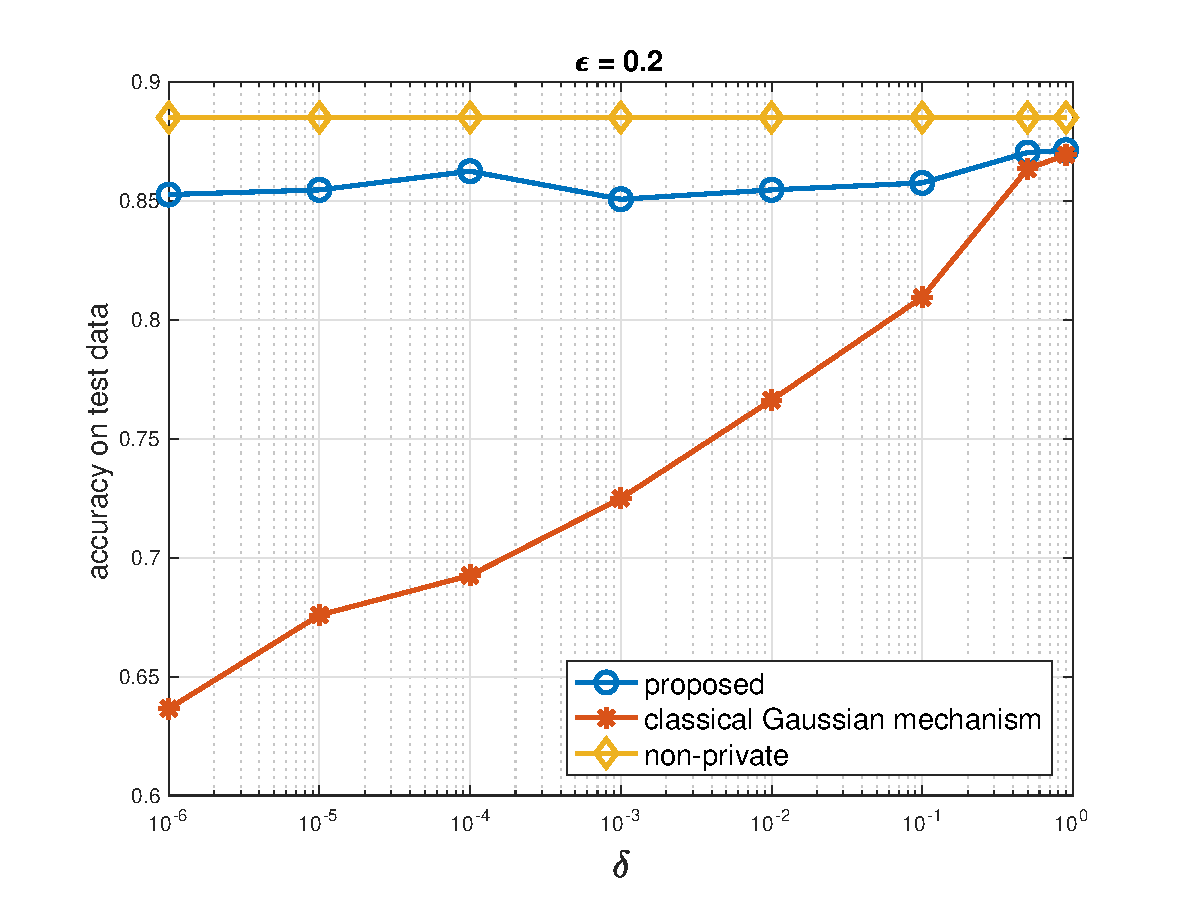
\includegraphics[width = 1.5in]{images/G_12}\label{fig_G_12}}}
% \centerline{ \subfigure[$\epsilon = 0.4$.]{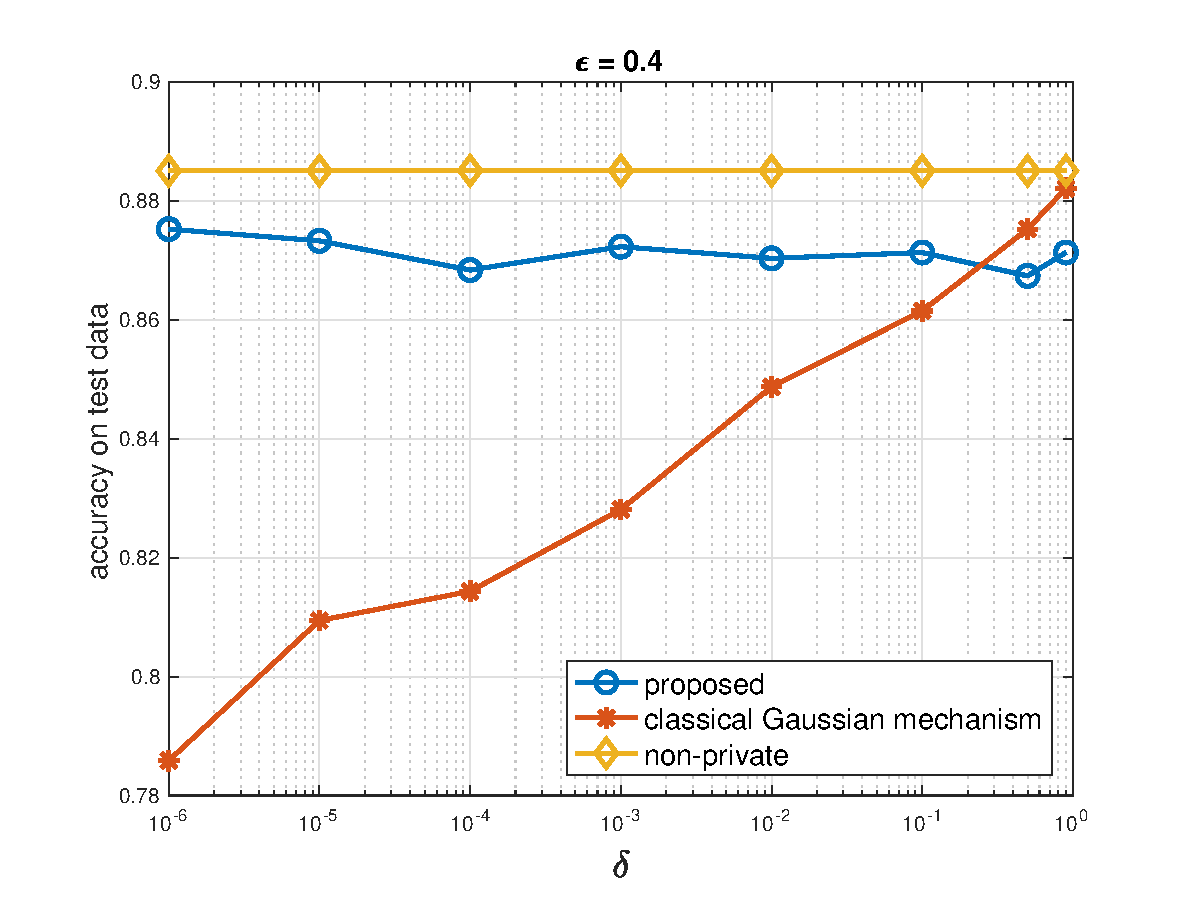
\includegraphics[width = 1.5in]{images/G_13}\label{fig_G_13}} \hfil \subfigure[$\epsilon = 0.6$.]{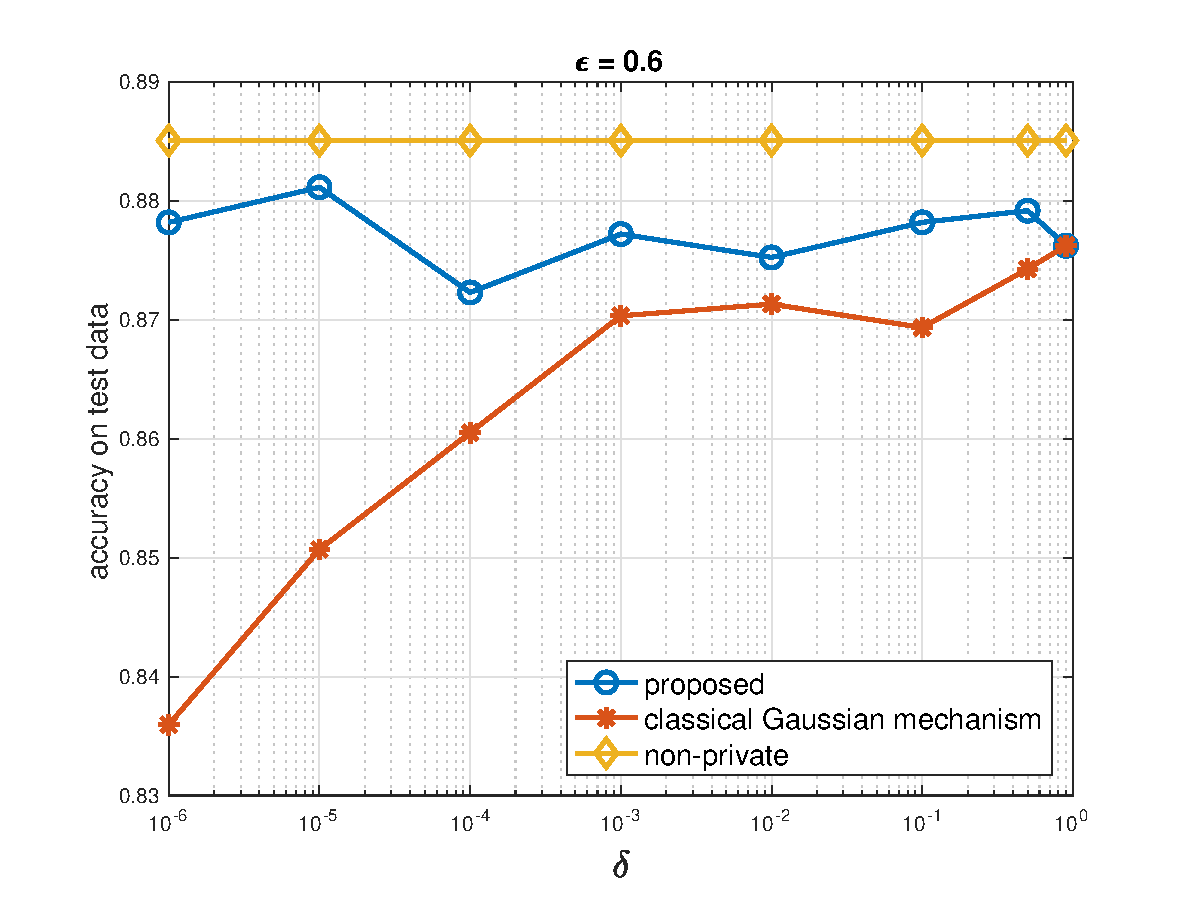
\includegraphics[width = 1.5in]{images/G_14}\label{fig_G_14}}}
% \centerline{ \subfigure[$\epsilon = 0.8$.]{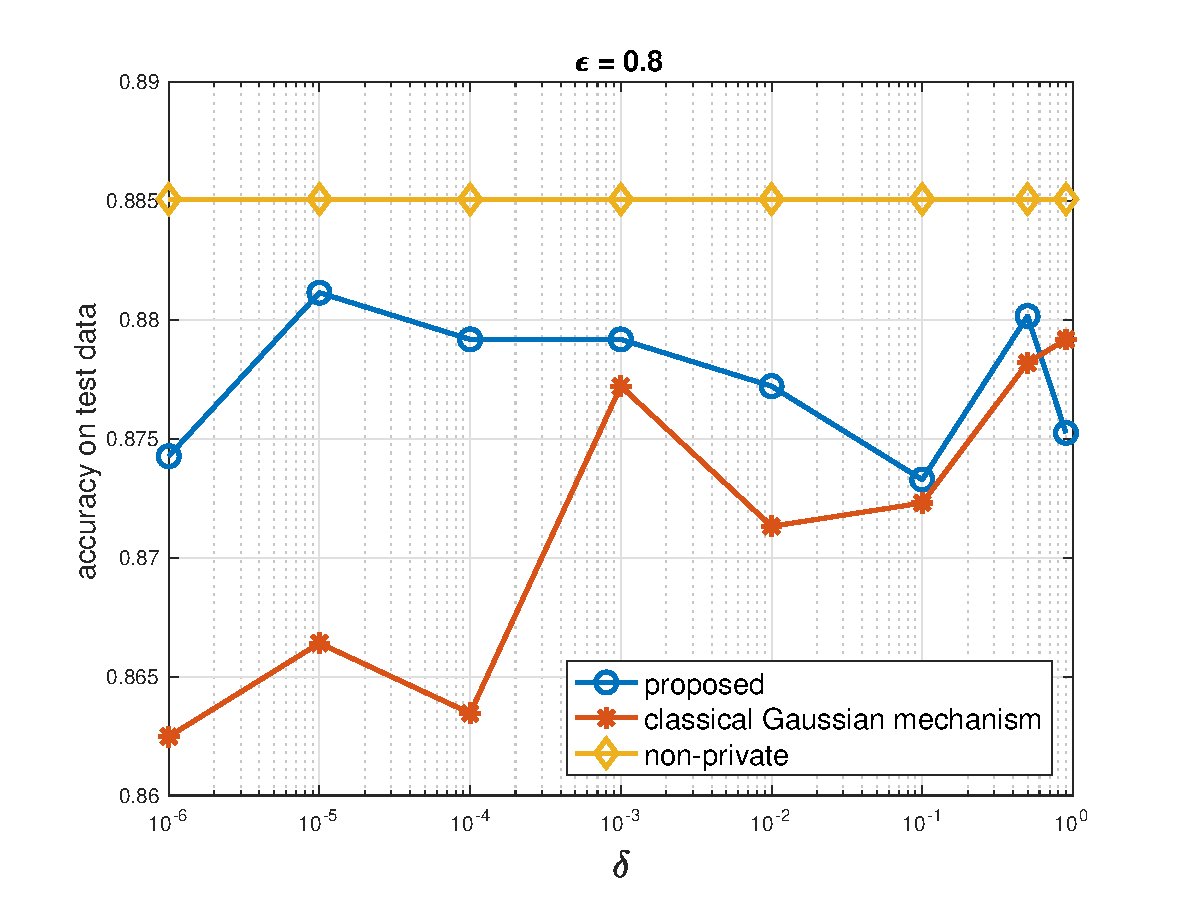
\includegraphics[width = 1.5in]{images/G_15}\label{fig_G_15}} \hfil \subfigure[$\epsilon = 1$.]{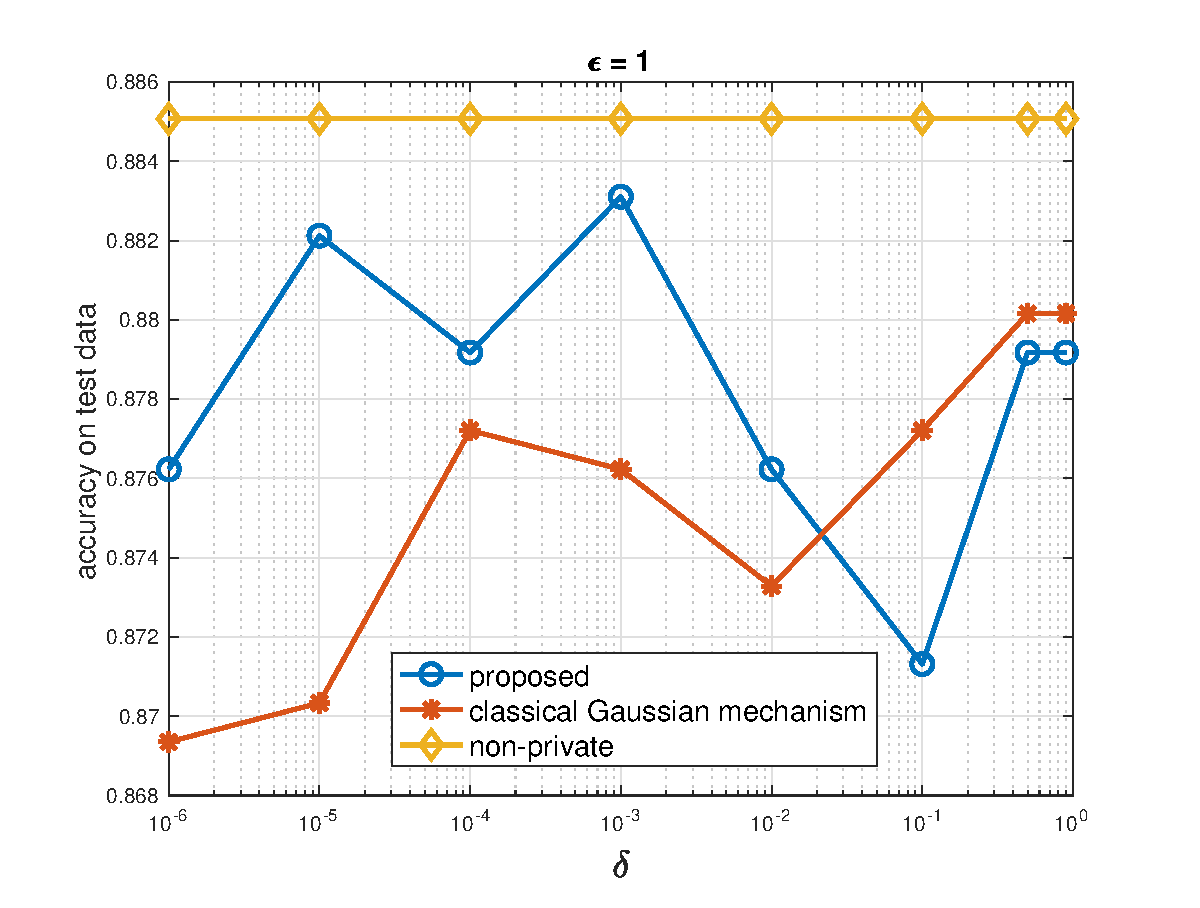
\includegraphics[width = 1.5in]{images/G_16}\label{fig_G_16}}}
% \caption{The effect of $\delta$ on Freiburg test data classification accuracy.}\label{fig_G_second_part}
% \end{figure} 
% \subsubsection{Caltech-101 Dataset}
% Catech-101~\cite{1384978} is a widely used dataset containing pictures of objects belonging to 101 categories. The dataset has 9144 images divided into 102 classes (101 object categories + one ``background'' category). Again, $8192-$dimensional feature vector is extracted from each image using AlexNet and VGG-16 followed by a normalization to have zero-mean and unity-variance along each dimension. As the classes have different number of images ranging from 31 to 800, we use a fixed number of training images per class and the classification performance is normalized across classes by calculating the average classification accuracy per class. The training set includes 30 randomly chosen images from each class and the rest images serve as the test images.
% \begin{table}
% \renewcommand{\arraystretch}{1.3}
% \caption{Results of experiments on Caltech-101 dataset}
% \label{table_results_caltech101} \centering
% \begin{tabular}{c||c}
% \hline
% \bfseries method  & \bfseries $\begin{array}{c} \mbox{testing accuracy in \%} \\ \mbox{(averaged per class)} \end{array}$   \\
% \hline \hline  
% $(0.1,1\mathrm{e}{-6})-$differentially private proposed & \textbf{87.20} \\
% $(0.1,1\mathrm{e}{-6})-$differentially private Gaussian & 36.92 \\
% Non-private proposed & \textbf{88.05}   \\
% Non-private SVM &    83.27      \\
% Non-private Naive Bayes &  83.24    \\
% Non-private Random Forest &  82.31    \\
% Non-private $1$-NN & 79.16    \\
% Non-private Decision Tree &  38.69  \\
% \hline \hline
% \end{tabular}
% \end{table}        

% The distributed learning scenario is created assuming that a class's complete training data is owned by a single participant. Thus, the number of participants is equal to 102. The method's $(\epsilon,\delta)-$differential privacy against perturbation (in one element of data vector), with perturbation magnitude upper bounded by $d = 0.1$, is studied. The experimental results have been summarized in Table~\ref{table_results_caltech101}. The results in Table~\ref{table_results_caltech101} further validate that    
% 1) The proposed optimal noise adding mechanism can result in multi-fold gain of the utility over the classical Gaussian mechanism. 2) The fuzzy based approach of this study offers a competitive alternative to the widely used machine learning methods for classification of high-dimensional data.

 
% \subsubsection{Caltech-256 Dataset}
% Caltech-256~\cite{griffinHolubPerona} is another challenging set of 30607 images labelled into 257 classes (256 object categories + one ``clutter'' category). A training set is built by choosing randomly 60 images from each of 257 classes and the rest images serve as testing set. The distributed learning scenario is created assuming that a class's complete training data is owned by a single participant. The method's $(\epsilon,\delta)-$differential privacy against perturbation (in one element of data vector), with perturbation magnitude upper bounded by $d = 0.1$, is studied. Table~\ref{table_results_caltech256}  reports the experimental results. The argument of competitive performance of proposed method is once again validated by the results stated in Table~\ref{table_results_caltech256}. 
% \begin{table}
% \renewcommand{\arraystretch}{1.3}
% \caption{Results of experiments on Caltech-256 dataset}
% \label{table_results_caltech256} \centering
% \begin{tabular}{c||c}
% \hline
% \bfseries method  & \bfseries $\begin{array}{c} \mbox{testing accuracy in \%} \\ \mbox{(averaged per class)} \end{array}$   \\
% \hline \hline  
% $(0.1,1\mathrm{e}{-6})-$differentially private proposed & \textbf{74.54} \\
% $(0.1,1\mathrm{e}{-6})-$differentially private Gaussian & 29 \\
% Non-private proposed & \textbf{77.25}   \\
% Non-private SVM &    69.24      \\
% Non-private Naive Bayes &  65.22    \\
% Non-private Random Forest &  63.66    \\
% Non-private $1$-NN & 61.64    \\
% \hline \hline
% \end{tabular}
% \end{table}    
\textbf{USTAN to provide the use case description and evaluation framework. Everyone to contribute once we have a clear idea about how to do evaluation}

%Need 2 to 3 pages on how we test serums?

{\color{purple}
Some thoughts/comments here:
\begin{itemize}
    \item Some evaluations will be from experts and some kinds of users (or through the use cases directly). These include areas like correctly being able to use the system, being able to authenticate well, etc.
    \item Some evaluations are ``formal'' in the sense that the goal is to use (semi-)formal methods to prove correctness. This includes the differential privacy, verification of components, modelling the system and showing results on the model, etc.
    \item We could consider compliance to be an evaluation criteria, e.g.~do we actually meet GDPR requirements.
    \item We may wish to link some of the above (or other) evaluation approaches to the KPIs we plan to have for the project.
    \item It may be helpful to link these to the earlier parts of the paper when done; e.g.~data fabrication is tested using technique X and shown that the fabricated and real data are indistinguishable.
\end{itemize}}

In this section, we present an initial evaluation of the \emph{Serums} technologies presented in Section~\ref{sec:technologies}. The evaluation was conducted on a data coming from a realistic use case, Edinburgh Cancer Data Gateway (ECDG), described in Section~\ref{sec:usecase}. In Section~\ref{sec:XX}, we show the ECDG data vault representing the smart patient record format. In Section~\ref{xx}, we show the synthetic data that was fabricated using the data fabrication technology, based on the format of ECDG data vault and additional corelations between fields of this format. We also verify how close the fabricated data is to the real data. In Section~\ref{xx}, we describe different access rights to the data, also demonstrating how blockchain can be used to regulate access based on these rights. In Section~\ref{XX}, we describe how the new authentication mechanisms can/will be used for the ECDG. Finally, in Section~\ref{xx}, we describe the application of privacy-preserving data analytics on the ECDG data, demonstrating increased privacy of the data while still being able to derive useful information from it.